\documentclass[a4paper, 11pt]{article}

%-------------------------------------------------------------------------------
%--- (a) Required Packages
%-------------------------------------------------------------------------------
\usepackage{amsmath,amsfonts,amssymb,amsthm}
\usepackage{adjustbox}
\usepackage{mwe}
\usepackage{authblk}
\usepackage[english]{babel}
\usepackage[para,online,flushleft]{threeparttable}
\usepackage{lscape}
\usepackage{threeparttablex}
\usepackage{tabu}
\usepackage{bm}
\usepackage{booktabs}
\usepackage{caption}
\usepackage{subcaption}
\usepackage[usenames, dvipsnames]{color}
\usepackage{epstopdf}
\usepackage[capposition=top]{floatrow}
\usepackage{framed}
%\usepackage[T1]{fontenc}
\usepackage{lmodern}
\usepackage{graphicx}
\usepackage{hyperref}
\usepackage[utf8]{inputenc}
\usepackage{lscape}
\usepackage{multirow}
\usepackage{natbib}
\usepackage{setspace}
\usepackage{rotating}
\usepackage{subcaption}
\usepackage{subfloat}
\usepackage{url}
\usepackage{wrapfig}
\usepackage{multicol}
\usepackage[toc,page]{appendix}
\usepackage{float}
\interfootnotelinepenalty=10000
\usepackage[margin=1in]{geometry}
\usepackage{textcomp}
\usepackage{longtable}
\usepackage{babel,blindtext}

%-------------------------------------------------------------------------------
%--- (b) Specific margins
%-------------------------------------------------------------------------------
%\setlength  \textwidth{\paperwidth}
%\setlength  \textheight{\paperheight}
%\setlength  \oddsidemargin{3cm}
%\setlength  \topmargin{-1.2cm}
%\setlength  \footnotesep{2ex}
%\addtolength\textheight{-6cm}
%\addtolength\textwidth{-6cm}
%\addtolength\oddsidemargin{-1in}
\setlength\parskip{0.25in} 
 
%%ADDED SPACE BETWEEN PARAGRAPHS 
%-------------------------------------------------------------------------------
%--- (c) Internal Ref stype
%-------------------------------------------------------------------------------

\hypersetup{            
    colorlinks=true,   
    linkcolor=Black,
    citecolor=BlueViolet,
    filecolor=BlueViolet,
    urlcolor=Black
}

 
%-------------------------------------------------------------------------------
%--- (1) Title
%-------------------------------------------------------------------------------
\title{The impact of abortion legalization on fertility and maternal mortality: New evidence from Mexico\thanks{We are grateful to Andreea Mitrut, Randi Hjalmarsson, Elin Larsson, Blair G. Darney, Hans Gr\"onqvist and seminar audiences at SOFI Stockholm University, Karolinska Institute and the CSAE conference for their very useful comments and discussions.  We thank Alejandro del Valle for sharing data, and Susanna Lindahl for excellent research assistance.}}

\author{Damian Clarke\thanks{Department of Economics, Universidad de Santiago de Chile.  Contact: damian.clarke@usach.cl} and Hanna Mühlrad\thanks{\textbf{Add full affiliaion} University of Gothenburg. Contact: hanna.muhlrad@gu.se}}

%-------------------------------------------------------------------------------
%---  ABSTACT
%-------------------------------------------------------------------------------
\begin{document}
\pagenumbering{gobble}
\maketitle
\newpage
\pagenumbering{arabic}

\begin{spacing}{2}
\begin{center}
  {\Large The impact of abortion legalization on fertility and maternal mortality: New evidence from Mexico}
  \\
\vspace{5mm}
  \textbf{Running Title}: Abortion Legalization, Fertility and Maternal Death \\
\textbf{Keywords:} Fertility, Maternal Mortality, Abortion legalization, Mexico

\end{center}

\newpage

\begin{abstract}
\noindent In this study, we examine the effect of a large-scale, elective, free abortion program implemented in Mexico City in 2007. Prior to this program, all states and districts in Mexico had very limited, or no, access to elective abortion. A localized reform in Mexico City resulted in a sharp increase in the request and use of early term elective abortions: approximately 90,000 abortions were administered by public health providers in the four years following the reform. We provide evidence using national vital statistics from Mexico suggesting that access to legal and safe abortion procedures result in decreased fertility and lower rates of maternal mortality. The difference-in-difference estimates suggest that this program resulted in a reduction in births by 2.3 to 3.8\% among women aged 15-44 and by 5.1 to 7.4\% among teenage women aged 15-19. Similar results are found for maternal mortality, for which we find a sharp fall in the rate of maternal deaths, by 11.1 to 20.0\% for women aged 15-44 and by 19.0 to 37.6\% among teenagers (15-19 years old).  
\end{abstract}

%\noindent \hspace{7mm} \textbf{JEL Codes:} I15, I18, O15. 


%-------------------------------------------------------------------------------
%---  INTRODUCTION
%-------------------------------------------------------------------------------
\newpage 
\section{Introduction}


 	
The issue of abortion legalization continues to be a highly controversial public health topic. This is especially true for Latin America, which exhibits some of the world’s most rigid and conservative abortion laws \citep{UN2014} as well as the highest estimated rates of unsafe\footnote{Unsafe abortion is defined as \textit{``a procedure for terminating an unintended pregnancy carried out either by persons lacking the necessary skills or in an environment that does not conform to minimal medical standards, or both''} \citep{WHO2011}.} abortions in the world, with 31 abortions per 1,000 fertile-aged women (ages 15-44) compared to the worldwide rate of 14 per 1,000. The high number of unsafe abortions in the Latin American and Caribbean (LAC) region corresponds to an estimated 4.2 million unsafe induced abortions each year. It is further estimated that these procedures account for 12\% of all maternal deaths in the LAC region \citep{WHO2011}.  Legal restrictions and low accessibility to contraceptives are the main causes of unsafe abortions, and unsafe abortions are a significant predictor of maternal death (see for instance \cite{Grimes2006}). This implies that the legalization of elective abortion could serve as an effective measure to reduce rates of maternal mortality. 


The ongoing public debate on abortion legalization continues to flare, not least in connection with the recent outbreak in Brazil of the ``\textit{Zika virus}'', which is thought to lead to microcephaly among infants \citep{heymann2016zika}. Some groups of lawyers, doctors, activists and UN spokesperson Cecile Pouilly have called on the Supreme Court of Brazil to allow for induced abortions \citep{guardianFeb}. When looking at the LAC region, there has been a development towards a more liberal abortion legislation in several South American countries, while opposite trends have followed in Central America (see \cite{Fraser} for an extended discussion). Similarly, differences in abortion laws can also be found on a sub-national level, which is the case for Mexico City where elective abortion during the first trimester was legalized in 2007.  

In this study, we use a local abortion reform in Mexico City and document the effect of free access to legal and safe abortion services on fertility and maternal mortality. While many studies in the economics literature\footnote{See for instance \cite{ananat_abortion_2009}, \cite{AngristEvans}, \cite{DonohueLevitt2001}, \cite{CharlesStephens2002}} have focused on the implications of the U.S Supreme Court decision, \textit{Roe v. Wade}, legalizing elective abortion in the US in 1973, we study abortion legalization in a developing country where the right to contraception is constitutionally protected. This reduced form analysis is carried out using Mexican vital statistics data from National Institute of Statistics and Geography (INEGI) on all registered births and maternal deaths during 2002-2011. The effect of the abortion reform is estimated using a quasi-experimental design, making use of state-level variation provided by the abortion reform. 


Abortion laws are determined at the state level in Mexico, where Mexico City (the federal district of Mexico) has its own legislative assembly. This reform provided all women who reside in Mexico City with access to legal and safe abortion procedures,free of charge and for any reason, during the first trimester. The law was a radical change to previous legislation in Mexico City, and compared to the rest of the states of Mexico, where abortion still is banned in all but extreme circumstances of rape, to save the mother's life, or in cases of fetal malformation. Moreover, by legalizing abortion, Mexico City distinguishes itself from nearly all countries in Latin America and the Caribbean which remain highly restrictive in their policies related to elective abortion.\footnote{According to the most recent United Nations figures \citep{UN2014}, Mexico is one of only three countries in the LAC region (along with Uruguay and Guyana) to be classified as the ``Least restrictive'' in abortion policy, implying that abortions are permitted for economic or social reasons on request.}
  

We find that providing access to safe and legal abortions free of charge resulted in a decrease in fertility between 2.3 to 3.8\% and a reduction in maternal mortality by 11.1 to 20.0\% among women aged 15-44. Our results show that there are heterogeneous effects across ages. We document a particularly strong effect among teenage women aged 15-19, for which our results suggest that the reform led to a 5.1-7.4\% reduction in fertility and a 19.0 to 37.6\% reduction in the maternal mortality rate. The decline in teenage fertility in Mexico City is consistent with the findings from abortion legalization (\textit{Roe v. Wade}) in the US, where an 8-12\% reduction in teenage fertility among non-white women and unmarried women was observed \citep{AngristEvans}. These findings are noteworthy given the high proportion of teenage motherhood in Mexico (18\% of all pregnancies are teenage pregnancies) and a well-documented negative association between teenage childbearing and education and labor market outcomes \citep{furstenberg1976unplanned}. 


Compositional changes among mothers are further examined and we find that, conditional on motherhood, the probability of teenage births decreases by 6.7\%, which further supports our previous finding of decreasing teenage fertility. We also find that the probability of having a first birth increases (compared to higher order births) and that the average age by parity (birth order) increases. Finally, the reform explicitly encouraged contraceptive usage by giving out contraceptives to women who accessed abortions as well as improved sexual education in schools. We use survey data from the Mexican Family Life Survey (MxFLS), containing information on contraceptive use and knowledge, to elaborate on potential channels through which the reform influences the outcomes. Our findings suggest that the main mechanism of reduced fertility and mortality is access to legal and safe induced abortion rather than other minor components of this program.   

Despite increasing attention being paid to rates of morbidity and mortality following unsafe abortion procedures \citep{Grimes2006,Brown2007,Kulczycki2011}, adequately measuring the impact of access (or lack thereof) to safe abortion is often hindered by poor and incomplete vital registration systems, and a paucity of appropriate (quasi-) experimental variation in access to safe abortion \citep{Grimes2006}. In this study however, we contribute to the existing literature by providing evidence of a causal relationship between access to legal abortion and fertility and maternal mortality in a developing country using vital statistics. Moreover, this is the first study to evaluate the overall effect on both fertility and maternal mortality from the 2007 abortion reform in Mexico City using the full set of available vital statistics for the period 2002-2011. Many previous studies examine the effect of abortion legalization that took place in conjunction with other major laws and reforms. In contrast to those studies, contraception has been legal and freely provided by the government since 1974 in Mexico.\footnote{The 2007 abortion reform in Mexico City brought improved sex education in schools as well as free access to contraception for women who had an abortion in a public clinic. However, the Mexican government has offered free access to contraceptives since the \textit{``General Population Law''} was passed in 1974 \citep{GIRE2009}.} Our results suggest that the 2007 abortion reform in Mexico City is associated with a reduction in fertility and maternal mortality. These results are highly relevant when considering the achievement of international development goals, including the Millennium and Sustainable Development Goals (MDGs and SDGs).


%%%COPIED FROM LITERATURE BELOW
%%There is a growing body of literature regarding reproductive health policies within economics. Abortion policy is a topic that has gained ground during recent decades, providing evidence of both short and long term consequences from abortion legalization and decriminalization. Within economics, there are a few proposed theoretical frameworks analyzing abortion policies and multiple empirical studies usually based on quasi-experimental methods.\footnote{From a theoretical point of view, suggested by \cite{levine2004abortion} and \cite{ananat_abortion_2009}, fertility decisions can be viewed as sequential choices of first becoming pregnant and then whether or not to give birth. Access to legal and safe abortion procedures decreases the “cost” of interrupting a pregnancy. This can imply two different effects on fertility decisions. First, better access to abortion reduces the probability of birth ex post becoming pregnant. Second, improved access to abortion can alter ex ante behavior and thus positively affect the number of pregnancies since opting out from pregnancy is less costly. However, due to lack of data on abortions prior to legalization of abortion, most studies analyze the effect on overall fertility while fewer study behavioral responses. In another theoretical paper by \cite{akerlof1996analysis}, the implication of legalizing abortion (and contraception)  is examined. They argue that abortion legalization causes more out-of wedlock births due to less shot-gun marriages. \cite{chiappori2008birth} provide a theoretical model and show, in contrast to \cite{akerlof1996analysis}, that access to birth control methods (including abortion) increases women's welfare and ``power''.} There are several studies with empirical evidence showing that abortion legalization has a negative effect on birth rates. One of the most studied abortion policies, is the US Supreme Court decision in the 1970s (Roe \emph{v.}\ Wade) legalizing elective abortion in all states.\footnote{See for instance \cite{ananat_abortion_2009}, \cite{AngristEvans}, \cite{DonohueLevitt2001}, \cite{CharlesStephens2002}} As a result of legalizing elective abortion, fertility decreased by 5\% with a particularly strong effect on teenage fertility, which declined by 12\% (see \cite{levine2004} for review). 

%%Similarly, a negative impact on fertility has also been found in former Soviet countries in Eastern Europe \citep{levine2004abortion}. Among these studies are \cite{Pop-Eleches}, who studied the 1966 Romanian ban on abortion during the rule of the communist dictator Ceausescu. The results show a radical increase in the total fertility rate (from 1.9 in 1966 to 3.7 children the year after). In contrast to the evidence from the US reform, women most inclined to access abortions before the ban were women with high socio-economic status. Analogous to previous findings, a large decrease in fertility by 8\% was found in Nepal when legalizing abortion \citep{Valente2010}.\footnote{In addition to short run effects, several papers examine the long run effect of abortion policies. From the US abortion policy, improved health and labor market outcomes have been found for the second generation. For instance, studies show improved outcomes in terms of lower child morbidity and mortality \citep{Gruberetal}, sharp decline in criminality \citep{DonohueLevitt2001}, more schooling and less welfare recipients \citep{ananat_abortion_2009} and reduced risk of substance abuse amongst adults \citep{CharlesStephens2002}. Similar results are found in Romania for the second generation. When controlling for various background covariates, infant mortality as well as later in life outcomes are worse for children born after the ban compared to those born prior \citep{Pop-Eleches} and \citep{Mitrut2011}.}

%%With regards to maternal mortality, there are multiple studies within the public health literature arguing that low accessibility to legal abortion causes higher incidence of maternal death and poorer maternal health outcomes.\footnote{Studies on maternal mortality are most common in the public health and medical literature, but also some studies within economics relating to this paper. For instance, \cite{jayachandran2008life} show a positive relationship between reduced maternal mortality and human capital investment amongst women in Sri Lanka and \cite{jayachandran2009modern} provide evidence of decreased mortality after introducing the sulfa drug in the US.} Amongst them are \cite{Singh2015}. By using data on abortion-related hospitalizations from six Latin American countries, an estimated 800 000 hospitalizations occur annually in Latin America, as consequences following unsafe abortions. A study by \cite{Grimes2006} uses a cross-country comparison approach examining the relationship between legal status of abortion and maternal health. They conclude that unsafe abortion is mostly common in countries where abortion is heavily restricted or illegal. They further show that morbidity and mortality related to complications from unsafe procedures are more predominant in places without legal access to abortion. Additionally, they emphasize that legal restrictions of abortion contribute to a substantial economic burden for the health care system, mis-allocating resources from other vital health care programs. Legal restrictions also generate indirect costs for society such as children growing up without mothers and deteriorating early childhood investments \citep{Grimes2006}. 


%%There are a number of studies which analyze the impact of the abortion legalization in Mexico using national vital statistics; \cite{Gutierrez2015} and \cite{Koch01022015}. Regarding the abortion reform and fertility outcomes, \cite{Gutierrez2015} use national vital statistics to examine the effect on fertility across ages. Due to the use of a limited amount of data and limitations inherent in the empirical design one cannot assign a causal interpretation to the results with confidence.\footnote{Only a limited amount of data is used comparing outcomes between three different years (1990, 2000 and 2010). Particularly, their ``double-difference'' coefficient is a simple comparison between 1990-2000 and 2000-2010, which is not a consistent way of using a difference in difference method (see for instance \cite{wooldridge2010econometric}), especially because the treatment group in not correctly specified when using the entire period 2000-2010 as the post treatment period while the reform took place in 2007} On the topic of the relationship between abortion legislation and maternal mortality in Mexico for the time period 2002-2011, \cite{Koch01022015} use national vital statistics and compare maternal mortality across states with ``less or more permissive'' abortion laws. However, the definition regarding ``less or more permissive'' abortion laws, used in  \cite{Koch01022015} leads to a misleading conclusion regarding the causal link between abortion legalization and maternal mortality.\footnote{Firstly, the treatment and control groups are incorrectly specified since the definition of abortion laws being “less or more permissive” are considered arbitrarily chosen (since abortion is only accessible in Mexico City and highly restricted elsewhere \citep{Kulczycki2011}). Secondly, \cite{Koch01022015} fail to account for lagged reporting of births by INEGI, resulting in more than 3 million incorrectly included births that took place before 2002. Thirdly, there is lacking information on the specification which has been used in this study. It does however appear that the treatment area is simply compared to the control area without using any methods that would provide results with a causal interpretation.} 

To the best of our knowledge, this is the first study to comprehensively document the effects of the 2007 abortion reform in Mexico City on both fertility and maternal mortality, heterogeneous effects across age with particular attention to teenage fertility and maternal mortality, compositional changes amongst mothers as well as suggestive evidence on potential mechanisms.          


\section{Mexican Context and the ILE Reform}
\label{reform}
The fertility rate in Mexico declined rapidly from roughly 6 children per woman in 1975 to nearly 2 in 2009. This major shift in fertility can be partially attributed to changes in access to modern contraceptive methods in the country \citep{GIRE2009}.  In 1975, the Mexican government passed the General Population Law, which obliged the government to supply family planning services and provide contraceptives via the public health care sector free of charge. Although 67\% of all women of childbearing age in Mexico report using modern contraceptive methods%\footnote{Modern contraceptives are condoms, oral or injectable or implants or hormones preventing ovulation, IUD, sterilization and emergency contraception. Traditional or less safe methods are calendar method or rhythm method, coitus interruptis, herbs or teas \cite{WHO2011}.}
(and 5\% use traditional and less safe methods), it is estimated that more than half of all pregnancies are unintended. Estimates suggest that up to 54\% of these unintended pregnancies are terminated \citep{GIRE2009}.

Mexico consists of 32 federal entities, 31 of which are federal states plus the federal district of Mexico (also known as Mexico D.F.\ or Mexico City).  As well as having a national constitution, each of the 32 federal entities has its own state or local constitution.  Abortion laws in all of Mexico are determined at the state level where Mexico City has its own legislative power, with the ability to regulate the abortion laws \citep{Becker}.  Mexico City contains approximately 8\% of the entire population (8.9 million of Mexico's 119.5 million inhabitants according to 2015 estimates) and is the only state that allows for elective abortion during the first trimester.  %In the online appendix to this paper, we provide further d In Figure~\ref{Map}, a map of Mexico is presented. 

Prior to the reform in Mexico City, abortion laws were rather uniform across the 32 federal entities of Mexico.  Induced abortion continues to be considered a criminal offense with the risk of legal consequence of up to 30 years imprisonment in many states \citep{GIRE2009}, and legal abortion was only permitted in the limited cases if rape, threat to the life of the mother, or severe malformation of the fetus.  In practice, even in these limited cases, legal abortion has been described by human rights organizations as extremely difficult to access due to rigid legal barriers \citep{GIRE2009}. In the densely populated Mexico City, only 62 abortions were legally performed during 2001-2007 \citep{Becker}. As a substitute to legal options, abortions were performed in clandestine and often unsafe settings. For example, in 2009 alone, medical records from public hospitals show that an estimated 159,000 women in Mexico were treated for abortion-related complications \citep{GIRE2009}.  The estimated national abortion rate in Mexico is 38 abortions per 1,000 women of fertile age \citep{GIRE2009}, which is considered high internationally \citep{Becker}. 

Due to the high number of unsafe abortions as well as a growing movement for women's reproductive health rights, the legislative assembly of the Federal District of Mexico City voted to legalize elective abortion (termed legal interruption of pregnancy, or ILE for its name in Spanish) on April 24, 2007, reforming Articles 145-148 of the penal code of Mexico City, and Article 14 of the Health Code.  These reforms were signed into law the following day.  A broader discussion of the reform's social and legal setting is provided in \citet{Kulczycki2011, Madrazo2009} and \citet{Johnson2013}.  This immediately permitted women above the age of 18 to request legal interruption of pregnancy at up to 12 weeks of gestation without restriction, while for those aged under 18, access required a parent or guardian's consent. The law included public provision of abortion procedures free of charge for women with residency in Mexico City at a selected number of public health clinics operated via the Ministry of Health in Mexico City (MOH-DF)\footnote{The public health care sector in Mexico is divided at both federal and state level, where the Ministry of Health (MOH) in Mexico City provides abortion procedures at a selected number of MOH-DF hospitals. Other MOH facilities (federally or state funded) are not legally required to provide abortion procedures.}.  Additionally, under this law, sexual education in schools was improved and post-abortion contraceptives were made freely available by the public sector \citep{Contreras2011}. Records from public hospitals show that the demand for post-abortion contraceptives is high (approximately 82\% of all women accept contraceptives) and that prevalence of repeated abortion procedures are low \citep{Becker}.

On August 29 in 2008 this decision was ratified by the Supreme Court of Mexico. The abortion reform in Mexico City is distinguishable as a major social and political reform and makes Mexico City, together with Cuba and Uruguay, the most liberal jurisdiction in terms of abortion legislation in the entire Latin American and Caribbean region \citep{Fraser}.

Women with residency outside Mexico City can also access the public provision of abortion through MOH-DF but are charged with a sliding fee scale determined with regard to the woman's socioeconomic background. In 2010, 74\% of all women who received an abortion through the public health care were women living in Mexico City, 24\% were living in the state of Mexico (which shares a border with Mexico City) and 2\% were living in other states \citep{Kalb}.  Figures from the Secretary of Health's administrative data suggest that abortions were used by women of all ages, though were dispoportionately sought by younger (21-25 year-olds) and older women (36 year-olds and above), with lower rates of abortion among 26 to 35 year olds.  The proportion of all births by age and all abortions in public health clinics by age is presented in figure \ref{MexBirthAbort}.

The law also allowed for private clinics to provide abortion services. Information regarding the private provision of abortion services is limited due to the lack of supervision of the private market for legal abortion services \citep{Becker}. During the year of 2007, (when the reform was implemented), more than 7,000 abortion procedures were performed at 14 selected MOH-DF clinics. Over the years, the MOH-DF abortion program expanded its services and became more efficient (shifting from surgical abortion procedures to medical procedures) at meeting the high demand for elective abortion. As of 2012, approximately 90,000 abortions have been carried out at the MOH-DF clinics \citep{Becker}, with no significant complications reported.

\section{Data}
\label{scn:data}
To examine the effects on fertility and maternal mortality, we use vital statistics on all births and maternal deaths in Mexico for the time period 2002-2011. The data is provided by the National Institute of Statistics and Geography (INEGI for its name in Spanish) and covers 23,151,080 live births and 11,858 maternal deaths among women aged 15-44.  Vital statistics for births in Mexico are compiled by INEGI based on birth registries completed by each parent or guardian at the civil registry, rather than being based on birth certificates issued at hospitals (as is the case, for example with the National Vital Statistics System in the USA).  Using data from the 2010 census and birth records up until 2009, recent (backward looking) analysis suggests that 93.4\% of all births in Mexico were registered within 1 year of birth of the child, and in total, 94.2\% of birth are eventually registered at the national level \citep{INEGI2012}.  The birth register is released once per year, containing all births \emph{registered} in that year, as well as the year of birth.  In order to avoid problems of under-reporting, differential reporting over time, and double-reporting, we collate all birth registries between 2002-2014, and then keep all births registered within 3 years of the date of birth.  This implies that we only have complete birth registries based on birth year up to (and including) 2011.  Maternal death data is taken from INEGI's full mortality register, which officially classifies maternal deaths according to ICD-10 codes and the World Health Organization's definition (see the data section of the online appendix for full details).  Mexico's registry of maternal deaths is recognised to be of high quality, with Mexico being classified as belonging to the ``A-class'' \citep{WHO1987} in the latest WHO report on maternal mortality trends.  This data has had particular improvements from 2002, and as such, we restrict our period of analysis to 2002 and beyond (see \citet{Schiavonetal2012} and the online appendix to this paper for further details).  

In the online appendix (table A-XXXX), we display the number of births and maternal deaths recorded in each federal entity over the period of study. Data from the birth and death registers is aggregated by each age group between 15-44, state, and year, resulting in a total of 9,600 cells (years$\times$states$\times$age). The INEGI Birth Register contains information about the date of birth, actual birthplace and the official residency of the mother. In addition, information on maternal characteristics such as age, birth order, educational attainment, marital status and employment status are recorded. The death register has a similar structure to the birth register and also records background information on the deceased women.

We then merge a range of time-varying covariates with birth and death data for each, year and state group described above.  This includes the population of women (variation by age, state and year) from the National Population Council of Mexico (CONAPO), socioeconomic variables including illiteracy, schooling, and access to health insurance from National Institute for Federalism and Municipal Development (INAFED) and the National Education Statistical Information System (SNIE), and data on the municipal-level roll-out of the national health insurance program \emph{Seguro Popular}\footnote{Mexico's General Health Law underwent a major reform in 2003, which intended to provide 50 million Mexican citizens, lacking social security, with subsidized and publicly financed health insurance. The core of this reform was the health insurance program \textit{Seguro Popular} (SP). The ``\textit{People’s Insurance}'' or \textit{Seguro Popular} was launched in 2002, offering health service free of charge or subsidized to those without formal health insurance. By 2005, two years before the reform, all 32 states had enrolled the SP program \citep{knaul__2007}.} from the INEGI data bank.  Socioeconomic data and measures of \emph{Seguro Popular} coverage vary by state and year.  We provide further details of data access and construction in the online appendix.

Summary statistics are presented in table \ref{sumStat2}.  In the top panel we present state-level characteristics, and in the bottom panel, individual characteristics from the vital statistics registries.  Unsurprisingly, there are relatively large differences between the densely populated Mexico City and the nearby state of Mexico and the rest of the country.  Residents of Mexico City have higher education and better access to health care. There are also substantial differences in the age composition, where mothers in Mexico City are, on average, older especially when having their first and second child.  Women dying from maternal mortality are on average less educated compared to the mean: a pattern observed in all areas of the country.  Turning to rates of maternal death and births per woman XXXX and make sure (and cite) that this agrees with official published stats XXXX.

\section{Empirical Strategy} \label{methodology}
The impact of the abortion reform is evaluated by using the subnational variation in abortion laws, and thus the access to legal and safe abortion procedures resulting from the ILE reform.  Given the temporal- and geographical-variation in availability of free legal abortions, we estimate the following difference-in-differences (DiD) specification:
\begin{eqnarray}\label{eq1}
	\text{Outcome}_{ast}= \beta_0 + \beta_1 \text{ILE}_{st} +\beta_2 \text{CloseILE}_{st}+ \bm{X}_{st}\bm{\delta} +\alpha_{s} + \nu_{t} +\pi_{a}+ \lambda_{s}\cdot t +\varepsilon_{ast}   
\end{eqnarray}
where Outcome$_{ast}$ represents our dependent variable of interest (fertility or maternal death) for age group $a$ in state $s$ and year $t$.  The treatment variable is determined by the official residency of the woman and indicated by ILE$_{st}$, which takes the value of one in Mexico City nine months after the ILE reform was adopted in order to compensate for the lag caused by the pregnancy length (assuming 40 weeks of gestation) and zero otherwise.\footnote{We choose the most conservative definition of the post-treatment period starting in January 2008 and onwards for our baseline specification. A more detailed description of the definition of treatment is provided in the online appendix, particulary table AXXXX.  As a robustness check, we use data at a monthly level and control separately for the partially treated births and maternal deaths and show that these results are consistent with our baseline results (online appendix table AXXXX).} As discussed in the previous section, a non-negligible proportion of all elective abortions i were accessed by women with residency in the neighbouring state of Mexico. Thus, to account for the potential spillover effects of the reform, we seperately control for this using the binary variable CloseILE$_{st}$ (equal to one in the state of Mexico nine months or more after the reform was passed and zero otherwise). 

The difficulty in evaluating effects of a new law lies in the fact that legislative changes often are endogenously determined.  That is, abortion legalization is likely to be correlated with observed and unobserved characteristics of Mexico City.  Even though the distribution of treatment is non-random, the inclusion of state ($\alpha_a$), year ($\nu_t$) and age ($\pi_a$) fixed effects allows us to estimate the impact of the reform in a so called difference-in-difference setting.  Under the parallel-trends assumption that in the absence of the reform treated and untreated states would have followed similar trends over time, DiD gives the causal impact of the reform on outcome variable.  We examine the veracity of this assumption in following sections.  In certain specifications, we include a full set of state-level time varying controls $\bm{X}_{st}$, and also allow for differential linear time trends in each state over time, captured by the $\lambda_{s}\cdot t$ terma.  The idiosyncratic error term $\varepsilon_{ast}$ is clustered at the state level in order to allow for autocorrelation of unobserved shocks within states over time\footnote{This is the generally accepted method in a DiD model \citep{Bertrandetal2004}.  However, there is a potential inconsistency in the standard error caused by serial correlation when the time period is long and numbers of groups (i.e. states) are small \citep{Bertrandetal2004}.  A likely outcome in these circumstances is underestimated standard errors leading to falsely significant difference in difference estimates.  This raises concern, since the number of clusters in our case are 32, which is slightly below commonly accepted ``rule of thumb'' thresholds for consistent estimation of standard errors \citep{angrist_mostly_2009,CameronMiller2015}. One suggested way of dealing with this problem is to use wild bootstrapped standard errors \citep{Bertrandetal2004,CameronMiller2015}, and as such, we also examine our main specifications using wild bootstrapped standard errors.}, and age by state by year cells are weighted by the state population (see for example \citet{Dell2015} for a discussion).

In our main specifications, births are measured as the log number of total births occurring in each cell.  While births can be measured in a number of ways, including counts, gross fertility rate and total fertility rate (which we report in the online appendix), we prefer the logged number of births for a number of reasons.  Firstly, we lack high quality yearly register data on population and are constrained to national representative survey data collected every five years and linearly interpolated for the years in between.  Secondly, we estimate regressions with log births using ordinary least squares (OLS) regressions.  Without the log normalisation of births, regression residuals are not normally distributed, and predicted values are at times negative.  Taking the log transformation allows us to resolve these issues in our case.

In contrast to the birth data which is strictly positive in all cells, the data on maternal mortality has a large number of cases where zero deaths are observed.  In our main specifications for maternal deaths, we estimate using the count of maternal deaths as the dependent variable, and use a Poisson regression model (estimates using the maternal mortality ratio and OLS are presented in the online appendix).%\footnote{A main assumption is thus that the number of events taking place during (non-overlying) time periods is independent of each other. That is, once a mother dies the deceased mother exits the process. While this assumption is likely to be satisfied for maternal mortality, this is not necessarily the case for fertility. Instead, for fertility this assumption may not hold because family planning methods are widely used for birth-spacing and it is not uncommon that births are explicitly timed apart or together.}
When using Poisson regression, the log average number of maternal deaths is modeled as a function of explanatory variables ($\log(\mu) =x\beta$), and taking the exponential of estimated coefficients gives the incidence rate ratios (porcentual effect) corresponding to the reform.

\section{Results}\label{scn:results}
\subsection{The effect of the reform on fertility and maternal mortality}\label{main}
In the main analysis, we estimate the effect of the reform using 1) the full sample of women aged 15-44 and 2) the subsample of adolescent women aged 15-19. We are interested in the overall effect from the reform on fertility as well as the effect on adolescent fertility. The reason for this is that the proportion of teenage childbearing in Mexico is very high (approximately 18\% of all births are teen births) and that teenage motherhood is correlated with worse outcomes in terms of education and poverty (see for instance \citep{furstenberg1976unplanned}.) 

The main results for fertility are presented in Table~\ref{MainRegBirth}. This table displays the difference-in-difference estimates from OLS regressions weighted by population, as specified in Equation~\eqref{eq1}, reflecting the effect of the abortion reform on fertility. The fertility outcome variable is the log number of births and we examine the effect on the full sample (column 1-5), as well as the subsample of adolescent women aged 15-19 (column 6-10). The effect on overall fertility and teenage fertility is estimated by first running a simple difference-in-difference specification excluding state specific linear time trends and time-varying controls (column 1 and 6). Then, trends (column 2 and 7) and time-varying controls (economic, education and health factors) are included gradually (column 3-5 and 8-10). These results suggest that the reform for women with residency in Mexico City led to a highly significant reduction in overall fertility, with a particularly strong effect on teenage women. For the full sample (women ages 15-44), the abortion reform is associated with a decrease in number of births by 2.3-3.8\% (column 1-5). The estimates for teenage women imply that the abortion reform is associated with a reduction in number of births by 5.1-7.4\%. 

These results imply that the reduction in fertility is close to double in magnitude compared to the overall effect. This is interesting because, while teenage childbearing is to a larger extent unintended, women below age 18 can only access legal abortions with parental consent (which introduces multiple decision makers and a possible barrier). For women with residency in the state of Mexico (the neighboring state to Mexico City), we don't find a significant impact of the reform, except for the simple diff-in-diff point estimate for teenage women (column 6). 

The difference-in-difference estimates from Poisson regression, specified by Equation~\eqref{eq1}, are presented in Table~\ref{MainRegMMR}. The outcome variables are number of maternal deaths by age, state and year and all regressions are weighted by number of births. Analogous to the estimation of the fertility outcome, state-specific linear time trends and control variables are included gradually. The point estimates for the full sample of women aged 15-44 (column 1-5) show that the abortion reform is associated with a significant decline in maternal mortality by 11.1 to 20.0\% (the effect size is calculated by exponentiated coefficients i.e exp($\beta$)-1 and can be interpreted as the incidence rate ratio). For teenage women aged 15-19 (column 6-10), the point estimates suggests a reduction between 19.0-37.6\%. The effects for teenage women are doubled in magnitude compared to the full sample but are only marginally statistically significant when including trends and state level controls. For women living close to the reform area (i.e in the State of Mexico), a significant effect from the reform is found for the full sample and teenage women when not including trends and controls.  

By including trends and time varying controls (columns 2-5 and 7-10), the magnitude of the coefficients increases. This suggests that the control variables are negatively correlated with the outcome variable and/or the explanatory variable. Moreover, the results indicate that the inclusion of time-varying controls of economic indicators affect the coefficient the most compared to indicators for education and health insurance. Because educational attainment could potentially be an outcome of the reform, we use proportion of illiterate population and the percentage of population aged 6-14 who are not enrolled in school. Moreover, the results are robust to the inclusion of the roll out of the national health care program Seguro Popular as well as controlling for the proportion of the population without health insurance. 

When interpreting the magnitude of the effect size from the reform it should be noted that the reduction in maternal deaths can be partly attributed to the overall decrease in fertility (as maternal deaths are mechanically a function of fertility), selection of mothers, as well as a lower rate of clandestine abortions.\footnote{The decrease in maternal mortality can be offset by lower incidence of unsafe abortions. The WHO predicts that 12\% of all maternal deaths can be accredited to unsafe abortions. Moreover, maternal mortality is automatically offset by lower fertility, since carrying out a pregnancy full term is always associated with mortality due to complications during pregnancy and childbirth. Additionally, there might be selection mechanisms such that women with low socio-economic status (encountering a higher risk for pregnancy complications) would also be more prone to access abortions.} 

%The disadvantage with using numbers rather than rates and ratios however, is the possibility of different changes in the population across treatment and control area over time. This could potentially lead us to the wrong conclusion regarding decreased fertility due to the reform, whilst the effect actually originates from a change in the population. However, controlling for state-specific yearly time trends should to some extent reduce a potential bias by absorbing the differences in the development of population across states and time.  Moreover, we find that the effects from the reform on rates and ratios are similar to the main results once we control for state-specific linear trends and time in-variant factors (see section~\ref{robust}).


\subsection{Heterogeneous effects}\label{heteroSection}

Heterogeneous age-specific effects of the reform are further explored in order to investigate the extent to which there is heterogeneity across age in accessing elective abortion. The take-up rate of free access to safe and legal abortion can be different across ages. There are several plausible explanations for this. First, some ages are more fertile than others, which can explain differences in usage. Second, attitudes and preferences can differ across ages. Third, women who were not able to have an induced abortion before the reform due to budget constraints can with the reform access abortions free of charge. This may particularly apply to teenage women, who are more likely to be financially constrained since they usually lack their own income or resources. For that reason, one could anticipate a more substantial effect on teenage women compared to older women. 

For this analysis, the full sample is divided into subsamples of the following age intervals: 15-18, 19-24, 25-29, 30-34, 35-39 and 40-44\footnote{Age-specific fertility is commonly divided into similar age intervals, see for instance \textit{2015 Revision of World Population Prospects}. Women below the age of 18 need parental consent for accessing elective abortion at public health facilities. We therefore group together women that need parental consent since the impact could differ for this specific group.} and we estimate the effect for each subsample according to the baseline specification (Equation~\eqref{eq1}).  State specific linear time trends and controls are included in each regression. The results from the heterogeneity analysis across age groups are displayed in Table~\ref{heteroReg}. 

In Table~\ref{heteroReg:1a}, the results for fertility are presented. As previously, the outcome for fertility is the log number of births and regressions are estimated using OLS. The results show that there are heterogeneous effects from the abortion reform across age groups. The reduction in births is highest among teenage women (15-18, column 1) with a decrease by 8.7\%. For the most fertile age groups (women aged 19-24 and 25-29, column 2-3), no significant effect is found. However for women aged 30-34, 35-39 and 40-44 (column 4-6), the abortion reform is associated with reduced fertility by 6.2, 4.7 and 3.6\% respectively. For women with residency in the State of Mexico, a significant effect (-2.5\%) is only found for women aged 35-39.   
  
In a similar manner, heterogeneous effects on maternal mortality across ages are presented in Table~\ref{heteroReg:1b}. As previously, the effect size is calculated by exponentiated coefficients i.e exp($\beta$)-1 and can be interpreted as the incidence rate ratio. Corresponding to the decrease in fertility, a large and highly significant reduction in maternal mortality, by 44.7\%, is found amongst teenage women 15-18. For women aged 19-24 however, the estimate is of opposite sign than would be expected. The strongest reduction in maternal mortality is found among women aged 25-29, with a highly significant reduction in maternal mortality by -49.8\%. The results further suggest a significant reduction in maternal deaths for women aged 30-34 and 40-44, by -32.5\% and -31.0\% respectively. No significant effect was found for women aged 35-39. Women under age 19 living in the State of Mexico experienced a similar reduction in maternal mortality to women with residency in Mexico City.  

The fact that the magnitude of effect in fertility and mortality does not exactly correspond to each other may depend on various selection mechanisms. That is, women dying from childbirth differ across multiple dimensions (for instance lower education etc) from women who have children, such that we don't necessarily expect an equal effect across the outcomes. 



\subsection{Parallel Trends and Placebo Testing}\label{parallel}



We recognize the fact that treatment is non-random and that Mexico City, the most urban and developed area of Mexico, may differ compared to other Mexican states across several dimensions. In the absence of parallel trends, the estimates would be biased and would lack a causal interpretation. Even though the results are robust to the inclusion of state-specific time trends and state level time-varying controls to account for potential differences in the changes of the dependent variable across time and states, this merely provides confidence in the results rather than explicitly test for the common trend assumption.\footnote{The identifying assumption can be formally described by:  
	\begin{equation*}
	E[\epsilon_{ast}|\alpha_{s},\nu_{t},X_{st}]=0.
	\end{equation*}.}

Trends in the main outcome variables are presented in Figure~\ref{Trends}. Even though the number of births differ in absolute levels between treatment and control area, changes in the number of births appear to be parallel by visual inspection prior to the reform, presented in Figure~\ref{birthTrends} and Figure~\ref{birthrateTrends}. For maternal mortality the variation is large and it appears rather difficult to draw conclusions from a visual inspection (see Figure~\ref{deathsTrends} and Figure~\ref{mmrTrends}). 

In addition to visual inspection of the pre-treatment trends presented in Figure~\ref{Trends}, two different tests are conducted. First, we examine whether the linear trend in the control group (i.e an interaction term between a linear time trend and the control group) for the pre-treatment period is statistically significantly different from the trend in Mexico City. The results are presented in Table~\ref{trendreg} in the Appendix, and show that the linear time trend for the control group is not statistically different from zero in the pre-reform period for either outcome. Secondly, to further investigate the common trend assumption, we conduct a full-event study in order to examine differences in trends in the pre-reform period for Mexico City and the control area. This is done by conducting a placebo test, in which we specify a similar specification as Equation~\ref{eq1} but rather than using a treatment variable for only the post reform period, binary treatment variables are included for each time period with the time period before the reform as the baseline period. We specify the following equation~\ref{eq2}:
\begin{eqnarray}\label{eq2}
  	Outcome_{ast}= \beta_{t} MexCity*time_{t}+	X_{st}\delta +\alpha_{s} + \nu_{t} +\pi_{a} +\epsilon_{ast}.   
\end{eqnarray}

  

 Equation~\ref{eq2} is analogous to Equation~\ref{eq1}; however instead of estimating the effect for the entire post treatment period in Mexico City, we use a more flexible model including interaction terms between Mexico City and all time periods (2002-2011) except for the time period just before the reform, which is the baseline category. We omit the State of Mexico due to potential spillover effects. The results are presented in Figure~\ref{placebo}. This procedure functions as 1) a placebo test: examining if there are any anticipatory effects, providing us with information if results are driven by pre-existing trends and 2) testing for parallel trends in the outcome variables: if trends are not common then this exercise would show significant estimates prior to the reform. The results show that there are no significant effects in the pre-reform period for log number of births, presented in Figure~\ref{placebo_birth}. A similar result  is found for the maternal mortality, displayed in Figure~\ref{placebo_mmr}, except for one pre-reform time period (first half-year of 2006) which exhibits a significant negative effect. From these exercises, we conclude that the placebo tests overall provide additional confidence in our results, with the exception of a decrease in maternal mortality in 2006.
 

   	  

\subsection{Spillover Effects}\label{Spillover}
As previously mentioned, potential spillover effects are problematic for estimating the impact of the reform, since a treated control group would bias the estimates.\footnote{Assuming that access to abortion leads to less children being born and less women dying from unsafe abortions, the estimates in presence of spillover effects would be downward biased. Even though data from the public hospitals show that, with exception of the neighboring State of Mexico, spillover effects are relatively small, we are still concerned that women living in places other than Mexico City would for instance access abortion procedures at private hospitals.} Under the assumption that spillover effects only occur in some of the untreated areas and not all, the treatment effect can be estimated consistently. This means that we can only estimate the effect of the abortion reform if spillover effects from the treated area are local. In addition, the common trend assumption must also hold for the partially treated areas.\footnote{See {\color{blue}{Clarke, 2015}} for an explicit and detailed analysis of estimation in the presence of spillover effects.} Moreover, we assume that the cost of traveling to Mexico City increases with the distance. This cost may consist of both actual traveling costs as well as other barriers that increase with distance from Mexico City such as social norms etc. Therefore  we assume that women living close to Mexico City are more likely to access the reform compared to women living further away. We estimate the following equation accounting for local spillover effects:

\begin{eqnarray}\label{eq3}
Outcome_{ast}= \beta_{1} Reform_{st} + \sum_{D}\beta_{D}CloseD_{st}\nonumber\\
X_{st}\delta +\alpha_{s} + \nu_{t} +\pi_{a}+ \lambda_{s}*time_{t} +\epsilon_{ast},
\end{eqnarray}
for $D\in \{0-5, 6-10, 11-15, \ldots, 51-55\}$.

This equation is analogue to Equation~\eqref{eq1}, with the exception of including multiple treatment variables equal to unity after the law was passed for states with the minimum distance $D$ within the distance intervals 0-5, 6-10, 11-15 up to 51-55 to Mexico City. There are 0-2 states within each distance interval. As in Equation~\eqref{eq1} we include age, year and state fixed effects in order to account for unobserved heterogeneity. In addition, we include state-specific time trends as well as state level time-invariant controls. We use an OLS regression for the fertility outcome and a Poisson regression for maternal mortality and the standard errors are clustered on state level.  


Figure~\ref{SpilloverFigure} confirms that there is no significant effect of the reform in states located within 0-5, 6-10, 11-15, $\ldots$, 50-55 km from Mexico City on either fertility (see Figure~\ref{spillover_birth}) nor maternal mortality (see Figure~\ref{spillover_MMR}). 



\subsection{Robustness}\label{robust}

A number of additional sensitivity and robustness checks of the main results on fertility and maternal mortality are conducted. We start out by using monthly data and examine if ignoring partially treated births and maternal deaths, when aggregating the data on yearly level, leads to biased estimates. While the full effect of the reform occurs with a nine month lag (40 weeks of gestational age) for fertility, a partial effect could occur already after six months since women who got pregnant between January 24 - April 23 in 2007 could, at least at some point during the first trimester, legally terminate their pregnancy.\footnote{For detailed description see Table~\ref{Exposure}.} This implies that the pre-reform period could be slightly contaminated when we conduct the analysis on a yearly level.\footnote{However, if we assume that fertility is negatively associated with abortion legalization, a partially treated control group would cause a downward bias in the estimates.} For this reason, we separately control for the partially treated births occurring between October and December 2007 and re-estimate our baseline specification using data on monthly level. The results are presented in Table~\ref{BirthMonth} in the Appendix and show very similar estimates for the fully treated births as to our baseline results. The estimates for the partially treated births are negative but insignificant and with lower magnitude compared to the fully treated births.   


In a similar manner, maternal deaths occurring after the reform was implemented, up until October 2007, could be partially treated. This was because  women whose unwanted pregnancy had reached beyond the first trimester could still choose to have an illegal abortion at a later point in their pregnancy (i.e the remaining six month of gestation). The partially treated women are therefore controlled for separately and the fully treated maternal deaths are defined as occurring after October 2007. The results are presented in Table~\ref{MMRMonth} in the Appendix and are similar to our baseline findings for the fully treated, but with somewhat smaller magnitude and lower precision. For the partially treated deaths, we don't observe any significant effect. In the regressions based on monthly data, estimates of the effect of the reform on maternal mortality have wider confidence intervals, as expected given the relative infrequency of these events and measurement challenges \citep{hogan2010maternal}. 


In the following sensitivity exercise, we re-specify the model according to Equation~\eqref{eq1} but instead of accounting for potential spillover effects by controlling for women with residency close to the reform we instead omit the State of Mexico from the analysis. The results are presented in Table~\ref{robust_reg:a}, and are robust for the fertility outcome, showing nearly no changes in the point estimates. However, the magnitude of the effect size is slightly lower compared to when we include a treatment variable for the State of Mexico. Additionally, we omit states in which more than 50\% of all births take place in rural areas (the eleven most rural states). That is, we worry that more rural and less developed states differ across various dimensions that cannot be controlled for. Table~\ref{robust_reg:b} presents the results from this exercise, which is very similar compared to the baseline results.     


We further analyze if the results are sensitive to alternative specifications by altering the measure of outcome variables and functional form. Again, we estimate the model expressed by Equation~\eqref{eq1} and presented in Table~\ref{Alternative}. First, we use the rate of birth as a measure of fertility presented in  column 1-5, Table~\ref{altspecRates}. Birth rate is defined as the annual number of births per 1,000 women for each age and state. Even though, the simple difference-in-difference estimate is surprisingly positive (and can be explained by differences in population trends).\footnote{Birth rates are calculated using linearly imputed data which seems to exhibits different linear trends for Mexico City and the rest of Mexico, the inclusion of state specific time trends are therefore important to include in order to estimate the causal link between the reform and birth rate.} On the other hand, once we control for trends and time varying state factors the point estimates of 2.0\% to 2.7\% (when the estimates are compared to the mean of the dependent variable), are similar in magnitude to the main results. Second, we estimate the effect on maternal mortality ratio (MMR), presented in column 6-10, Table~\ref{altspecRates}. MMR is defined as the annual number of maternal deaths per 100,000 live births for each age and state. The impact on MMR, with the effect size compared to the mean of the dependent variable of -5.8 to -22.9\% for women with residency in Mexico City, is similar to the main specification. In addition, we estimate the effect on number of births using OLS regressions presented in Table~\ref{OLS_levels} in the appendix. The results suggest that the precision and magnitude is somewhat lower compared to the main results. The overall results from this exercise provide a similar estimated effect of the reform for women aged 15-44 with residency in Mexico City when including state-specific linear time trends and time invariant controls. However, the results seem to be sensitive to altering the functional form and measure of fertility and mortality. 

In a difference-in-difference setting there is a potential inconsistency in the standard error caused by serial correlation when the time period is long and numbers of groups (i.e. states) are small \citep{Bertrand2002}. A likely outcome in these circumstances is underestimated standard errors leading to falsely significant difference in difference estimates. This raises concern, since the number of clusters are 32, which is slightly below the commonly accepted threshold for consistent estimation of standard errors \citep{angrist_mostly_2009}. One suggested way of dealing with this problem is to use wild bootstrapped standard errors \citep{Bertrand2002}. We re-estimate the main results for fertility and maternal mortality\footnote{Wild bootstrapping is not plausible for non-linear models. For that reason, we add the value one to all observations for maternal mortality and log transform the number of deaths.} using wild bootstrapping and conclude that the results\footnote{The estimates differs slightly compared to the baseline results because the implementation of this estimator using wild bootstrapping was incompatible with the use of population weights.} remain statistically significant below a 5\% level. The result is presented in Table~\ref{inference}. While this exercise might mitigate some concern regarding underestimated standard errors, the magnitude of this problem is yet difficult to assess, for that reason the precision of the results should be interpreted with some caution.    


\subsection{Compositional Changes}\label{CompositionalChanges}

Changes in the composition of mothers are further explored by using disaggregated data covering all births and maternal deaths. Provided the available data on maternal characteristics from the birth register, we can observe whether or not the reform affected fertility and mortality differently across various dimensions such as age, parity, age by parity and educational level.\footnote{The abortion reform may exhibit multiple contemporaneous effects on fertility outcomes and fertility decision making. Access to abortion may influence the total fertility as well as the timing of childbearing, for which the effect may be heterogeneous across the population affecting some women more than others. For example, legalizing abortion may reduce women’s total fertility and assist them in obtaining their desirable number of children, such that access to abortion would facilitate the transition from child quality to child quantity more easily \citep{becker1974interaction}. Moreover, access to abortion can also provide better opportunities for women to optimize the timing of reproduction. It is suggested that women with access to abortion can delay childbearing more efficiently and hence provide a better environment for their children with regards to the mother’s economic and social situation \citep{DonohueLevitt2001}. If this was the case, the total fertility could remain unchanged while children being born would be born under (relatively) better circumstances. Furthermore, these potential mechanisms may be stronger or weaker depending on socio-economic factors.} Specifically, we examine the effect on teenage fertility once more, using disaggregated data, comparing the proportion of teenage births to all births in a diff-in-diff manner.   
 

 Conditional on being a mother, we examine the effects of the reform on 1) the probability of teenage motherhood 2) the probability of giving birth to your first child or higher order births and 3) age by parity (birth order). By utilizing the information on maternal characteristics, we can analyze the age profile and number of children per woman accessing the reform. The results are displayed in Table~\ref{comp}. The difference-in-difference analysis shows that, conditional on motherhood, the reform decreases the probability of teenage motherhood by 6.7\% when comparing the estimate to the mean of the dependent variable (column 1). In column 2-4 the effect on parity (birth order) is examined. The results indicate that the probability of mothers giving birth to their first child increases slightly and decreases for the birth order being 2 or higher. However, these effects are insignificant. Age by parity is further explored and presented in column (5-7), and shows that age at second child increases slightly, while this effect is significant, the magnitude is very small. These results suggest that childbearing among teenage women decreases.  

 

 The effects of the reform on educational attainments conditional on motherhood are also analyzed. The results are presented in Table~\ref{educ_Birth_mmr} in the appendix. However, due to lack of common trends in the educational composition between the reform and non-reform states these results do not have a causal interpretation. The results suggest that those accessing the reform are mainly women with very low levels of education and women with high school education or above. These findings may suggest that there are selection mechanisms where low SES women and high SES women either decrease their fertility and/or alter the timing of childbearing. 
%%%% My preference then would be to just remove this part of the analysis.  Given that we say we don't believe it, we probably shouldn't present it.
 
 In a similar manner to the previous analysis, we examine the characteristics of deceased mothers by using data on all maternal deaths. While we lack information on birth order, the death certificates contain information on educational attainment of the deceased women.\footnote{However, there are no common trends in education attainment for the sample of decreased mothers, which challenges the causal interpretation of these results.} These findings (Table~\ref{educ_Birth_mmr} in the Appendix) suggest that the proportion of deceased mothers with primary education decreased due to the reform, while the proportion of deceased mothers with no education or professional education increased. These results contradict the results on educational attainment for the women who gave birth. However, the distribution of educational attainment of deceased mothers is very different from the distribution of educational attainment for mothers in general. It is therefore likely that the abortion reform would affect the composition of mothers differently. 

 
\subsection{Mechanisms}\label{Mechanisms}

The 2007 abortion reform had three components, of which the main component of the reform was legal access to safe and free abortion. However, the reform also called for improved sexual education in schools as well as access to free post-abortion contraceptives through the MOH-DF program \citep{Becker}. In this paper, we carry out a reduced form analysis of the impact of the reform. For this reason, we further examine possible mechanisms by which the reform affects fertility and maternal mortality by including state level information on contraceptive usage and knowledge in the baseline analysis. We use information regarding contraceptive knowledge as a proxy for the general information about family planning obtained.


In order to examine potential mechanisms through which the reform may have affected fertility and maternal mortality, we use data on contraceptive use and knowledge from the Mexican Family Life Survey (MxFLS), which was conducted in 2002-2003, 2005-2006 and 2009-2012 and covers 15,768 women.\footnote{Due to small sample size and the design of the survey we cannot divide the sample into sub-samples for teenagers or similar.} Data points between those years are generated by linear interpolation. For more information about the data set see section~\ref{mxfls} in the data appendix. We use the following definitions about family planning habits; \textit{the proportion of women aged 15-44 who report current use of modern contraceptives} and \textit{the proportion of women aged 15-44 who report current use of any type of (modern or traditional) contraceptive method}.\footnote{For a detailed description of modern and traditional methods see for instance WHO (2015).} Modern contraception methods include condoms, oral or injectable implants of hormones preventing ovulation, IUD, sterilization and emergency contraception. Traditional or less safe methods are the calendar method or rhythm method, coitus interrupts and herbs or teas. Information regarding modern contraceptive methods is used as a proxy of general information about family planning and is defined as \textit{the proportion of women aged 15-44 who report having knowledge about at least one modern contraceptive method}. 



The results are presented in Table~\ref{meck} and show the difference-in-difference estimates specified by Equation~\eqref{eq1}.\footnote{The sample size is smaller compared to the baseline because of missing values for some states} Column 1 presents the baseline results (see Table~\ref{MainRegBirth} and~\ref{MainRegMMR}) when controlling for a full set of fixed effects, state-specific trends and state varying economic, educational and health controls. In addition to the baseline specification, we include state-level information on current use of modern contraceptives (column 2), current use of any type of contraceptives (column 3) and knowledge about modern contraceptives (column 4). The estimates for fertility when including these variables respectively (-3.9\%, -3.5\% and -2.5\%) are similar to the baseline results (-3.8\%). The result of maternal mortality is analogous to the previous, for which the magnitude of the reform-coefficient (-23.7\%, -22.6\% and -27.3 \%) are similar to the baseline result (-23.3\%) when including state-level controls. 


The overall result for this exercise confirms the notion that the main channel by which fertility and maternal mortality are affected by the reform is by legal access to safe and free abortion procedures. Whilst we should take into consideration that data on contraceptive use and knowledge is obtained from three waves of survey data (and linearly interpolated for the years in between), these results indicate that we cannot rule out that the reduction in fertility and maternal mortality could mostly be attributed to free access of induced abortion services rather than minor components of the reform.\footnote{Similar results are found when using data from the Mexican National Health Survey (ENSA) and the Mexican National Survey of Health and Nutrition (ENSANUT). However, the data of contraceptive use and knowledge from this survey are inadequately measured due to inconsistent questions across waves. These results are available upon request.}

    

 
 
\section{Conclusion}\label{Conclusion}
In this paper, we examine the effect of abortion legalization on women's reproduction and health in Mexico City. The 2007 abortion reform in Mexico City was a major social and political reform, providing all women with residency in Mexico City access to safe elective abortion during the first trimester. Prior to the reform very few legal abortions were performed, although clandestine abortion was very common \citep{Becker} leading to a high number of women suffering from complications associated with unsafe procedures each year \citep{GIRE2009}. By using sub-national variation in abortion laws, we analyze the effect of the reform on fertility and maternal mortality using vital statistics from the National Institute of Statistics and Geography (INEGI) during the time period 2002-2011. 

We extensively document two main findings. First, the reform has a considerable effect on fertility rates, reducing births in Mexico City by between 2.3 and 3.8\%. Secondly, access to elective abortions significantly reduces maternal mortality by 11.1 to 20.0\%. These effects are especially strong among teenage women aged 15-19, with a decline in fertility by 5.1 to 7.4\% and in maternal mortality by 19.0 to 37.6\%. Moreover, our results suggest that the reform affected the composition of mothers. Conditional on motherhood, we find that mothers are 6.7\% less likely to be teenage mothers and a small effect on age by parity, where age slightly increases for the second child. In addition, we utilize survey data (MxFLS) regarding knowledge and use of contraceptives and investigate potential mechanisms. Our findings indicate that the main mechanism behind our results is free access to legal and safe induced abortion compared to other potential mechanisms.
 
The reduction in fertility indicates that despite the large number of risky clandestine abortions practiced prior to the reform in Mexico City, considerable unmet demand for contraception still remained. In the presence of high rates of teenage pregnancy and undesired births, the legalization of abortion was thus responsible for an important reduction in the number of births observed. Moreover, our maternal mortality results suggest that safe procedures in legal environments can have large impacts on the significant number of women who still die from complications due to unsafe abortion in Mexico. 
 
\end{spacing}
% % % % % % % % % % % % % % % % % % % % % % % % % % %
% % % % References % % % % % % % % % % % % % % % % % 
% % % % % % % % % % % % % % % % % % % % % % % % % % %
\newpage
\bibliographystyle{ecta}
\bibliography{refs}
\begin{spacing}{2}




%%%%%%%%%%%%%%%%%%%%%%%%%%%%%%%%%%%%%%%%%%%%%%%%%%%%%%%%%%%%%%%%%%%%%%%%%%%%%%%%%%%%%%%%%%%%%%%
%%% TABLES
%%%%%%%%%%%%%%%%%%%%%%%%%%%%%%%%%%%%%%%%%%%%%%%%%%%%%%%%%%%%%%%%%%%%%%%%%%%%%%%%%%%%%%%%%%%%%%% 
\section*{Tables}
\begin{table}[H]\caption{State and Maternal Characteristics}\label{sumStat2}
\begin{threeparttable}
{\small 	\begin{tabular}{lcccc}\toprule\toprule
		& (1) & (2) & (3) & (4) \\ 
  	& Mexico & State of & Rest of & Full \\ 
 	&City&Mexico&Mexico&Country \\ 
	
	
	\hline &&&&\\
		 \multirow{1}{*}{} &
		 \multicolumn{4}{c}{\textbf{\textsc{State Characteristics}} }\\\cline{2-5}
	 &&&&\\
 Birth rate & 64.7&85.7 &88.5 &86.0\\
 &(33.5)&(48.9)&(47.7)&(47.3) \\
	Maternal Mortality Ratio &  54.3&54.7 &50.3 &51.2\\
	 &(47.4)&(41.6)&(68.0)&(63.8) \\
	Illiteracy      &       2.409&       11.74&       8.756&       8.606\\
	&     (0.257)&     (1.202)&     (5.125)&     (5.104)\\
	
	People aged 6-14 with no schooling   &       2.951&       7.976&       5.373&       5.398\\
	&     (0.151)&     (1.005)&     (1.562)&     (1.706)\\
	
	No health rights    &       39.13&       59.74&       42.74&       43.52\\
	&     (4.334)&     (11.35)&     (15.47)&     (15.43)\\
 

	 &&&&\\
			 \multirow{1}{*}{} &
			 \multicolumn{4}{c}{\textbf{\textsc{Individual Characteristics}} }\\\cline{2-5}
 	\textbf{\textsc{\underline{Mothers}}}	&&&&\\
 	  
 	  Age & 26.51& 25.60&25.61 &25.66\\
 		&(6.235)&(6.064)&(6.146)&(6.145)\\
 	  Age at first birth& 24.71& 22.78& 22.72& 22.94  \\
 		&(6.140)&(5.620)&(5.453)&(5.559)\\
 		 
 	 
  Incomplete Primary&       2.123&       6.810&       13.06&       12.16\\
	&     (0.346)&     (2.150)&     (9.363)&     (9.273)\\
  Primary&       10.51&       20.60&       25.66&       24.62\\
	&     (1.937)&     (2.742)&     (6.207)&     (6.847)\\
 
  Secondary&       39.35&       44.70&       34.69&       35.48\\
	&     (0.750)&     (1.795)&     (7.704)&     (7.703)\\
  Preparatory&       28.93&       19.40&       16.68&       17.45\\
	&     (1.333)&     (2.339)&     (4.588)&     (5.153)\\
	
  Professional education&       19.08&       8.490&       9.911&       10.29\\
	&     (1.470)&     (0.847)&     (2.840)&     (3.397)\\
	 
  
 \textsc{\textbf{\underline{Deceased Mothers}}}		&&&&\\
 
 
  No Schooling &       2.049&       5.810&       10.60&       9.903\\
	&     (8.949)&     (14.64)&     (25.32)&     (24.36)\\
  Incomplete Primary &       18.44&       30.47&       35.45&       34.32\\
	&     (26.29)&     (27.00)&     (40.25)&     (39.22)\\
  Primary  &       10.25&       10.76&       10.18&       10.22\\
	&     (19.99)&     (17.69)&     (26.34)&     (25.64)\\
  Secondary &       32.05&       29.99&       24.27&       24.98\\
	&     (32.17)&     (24.51)&     (36.79)&     (36.05)\\
  Prepatory &       22.94&       14.59&       11.40&       12.15\\
	&     (29.17)&     (17.32)&     (27.04)&     (26.82)\\
  Professional education &       14.28&       8.380&       8.101&       8.426\\
	&     (24.28)&     (14.38)&     (23.06)&     (22.76)\\\hline
\textbf{N Births}& 1,505,790 & 3,186,751& 18,464,578& 23,157,119  \\ 
\textbf{N Maternal Deaths}& 818 & 1,745 & 9,295 & 11,858\\
\textbf{N States} & 1&1&30&32\\
 	\hline\hline
\end{tabular}}
 
 
 

\begin{tablenotes}
\item Note to Table~\ref{sumStat2}:	The data for state characteristics is obtained from the National Institute for Federalism and Municipal Development (INAFED) respectively the National Education Statistical Information System (SNIE). Maternal characteristics are obtained from administrative data made available by INEGI of all births and maternal deaths for women aged 15-44 during the time period 2002-2011. Proportion of the population in\%age and standard deviation in the parenthesis.
\end{tablenotes}
\end{threeparttable}
\end{table}



%%%%%%%%%%%%%%%%%%%%%%%%%%%%%%%%%%%%%%%%%%%%%%%%%%%%%%%%%%%%%%%%%%%%%%%%%%%%%%%%%%%%%%%%%%%%%%%
%%% REGRESSIONS
%%%%%%%%%%%%%%%%%%%%%%%%%%%%%%%%%%%%%%%%%%%%%%%%%%%%%%%%%%%%%%%%%%%%%%%%%%%%%%%%%%%%%%%%%%%%%%% 
\begin{sidewaystable}[H]\caption{Effects of the Reform on Fertility} \label{MainRegBirth}
\begin{threeparttable}
 {\footnotesize  {
\def\sym#1{\ifmmode^{#1}\else\(^{#1}\)\fi}
\begin{tabular}{l*{10}{c}}
\hline\hline
                    &\multicolumn{5}{c}{\textbf{Full-Sample 15-44}}                                 &\multicolumn{5}{c}{\textbf{Teenage women 15-19}}                               \\\cmidrule(lr){2-6}\cmidrule(lr){7-11}
                    &\multicolumn{1}{c}{(1)}&\multicolumn{1}{c}{(2)}&\multicolumn{1}{c}{(3)}&\multicolumn{1}{c}{(4)}&\multicolumn{1}{c}{(5)}&\multicolumn{1}{c}{(6)}&\multicolumn{1}{c}{(7)}&\multicolumn{1}{c}{(8)}&\multicolumn{1}{c}{(9)}&\multicolumn{1}{c}{(10)}\\
                    &\multicolumn{1}{c}{\shortstack{OLS\\Log\\ Num. of \\Births}}&\multicolumn{1}{c}{\shortstack{OLS\\Log \\Num. of \\Births}}&\multicolumn{1}{c}{\shortstack{OLS\\Log\\ Num. of \\Births}}&\multicolumn{1}{c}{\shortstack{OLS\\Log \\Num. of \\Births}}&\multicolumn{1}{c}{\shortstack{OLS\\Log\\ Num. of \\Births}}&\multicolumn{1}{c}{\shortstack{OLS\\Log\\ Num. of \\Births}}&\multicolumn{1}{c}{\shortstack{OLS\\Log \\Num. of \\Births}}&\multicolumn{1}{c}{\shortstack{OLS\\Log\\ Num. of \\Births}}&\multicolumn{1}{c}{\shortstack{OLS\\Log \\Num. of \\Births}}&\multicolumn{1}{c}{\shortstack{OLS\\Log\\ Num. of \\Births}}\\
\hline
&&&&&&&&&&\\
Reform              &     -0.0226** &     -0.0284***&     -0.0356***&     -0.0377***&     -0.0461***&     -0.0506***&     -0.0595***&     -0.0730***&     -0.0709***&     -0.0745***\\
                    &     (0.009)   &     (0.005)   &     (0.006)   &     (0.008)   &     (0.010)   &     (0.012)   &     (0.007)   &     (0.007)   &     (0.010)   &     (0.015)   \\
[1em]
ReformClose         &    -0.00924   &     0.00536   &     0.00102   &     0.00335   &    -0.00355   &     -0.0253** &     0.00894   &     0.00195   &   -0.000268   &    -0.00741   \\
                    &     (0.009)   &     (0.005)   &     (0.006)   &     (0.011)   &     (0.016)   &     (0.012)   &     (0.006)   &     (0.006)   &     (0.011)   &     (0.013)   \\
\hline
\(R^{2}\)           &       0.904   &       0.905   &       0.905   &       0.905   &       0.916   &       0.649   &       0.650   &       0.650   &       0.650   &       0.603   \\
Mean\_of\_dep\_Var     &       7.819   &       7.819   &       7.819   &       7.819   &       7.419   &       7.918   &       7.918   &       7.918   &       7.918   &       8.134   \\
Observations (State*Year*Age) & 9600&9600& 9600&9600&9600&1600&1600&1600&1600&1600\\
Number of women & 269189193&269189193&269189193&269189193&3930& 53570502&53570502&53570502&53570502&29523390\\
\hline State, Year and Age FE& \checkmark &\checkmark&\checkmark& \checkmark&\checkmark&\checkmark&\checkmark&\checkmark&\checkmark&\checkmark\\
State Specific Linear Trends&&\checkmark&\checkmark&\checkmark&\checkmark&& \checkmark&\checkmark&\checkmark&\checkmark\\
Economic controls&& &\checkmark& \checkmark&\checkmark&&&\checkmark&\checkmark&\checkmark\\
Education controls&&&& \checkmark&\checkmark&&&&\checkmark&\checkmark\\
Health controls&&&&& \checkmark&&&&&\checkmark\\\bottomrule\bottomrule
\end{tabular}}
}
\begin{tablenotes}
\footnotesize
\item \textit{Note to Table~\ref{MainRegBirth}}. The table displays the difference in difference estimates from OLS regressions. The sample consists of all births among women aged 15-44 (column 1-5) and sub-sample of teenage women aged 15-19 (column 6-10), for the period 2002-2011. The dependent variables are defined as the log number of births. The independent variable \textit{Reform} takes the value 1 in Mexico City 9 months after the law was passed due to realization of gestation and 0 otherwise. Similarly, \textit{ReformClose} is a binary variable equal to 1 in the neighboring State of Mexico 9 months after the reform was introduced. The economic controls are state level income, unemployment and rurality. The educational controls are illiteracy and proportion of people aged 6-14 who are not enrolled in school. The health controls are the proportion of residents with no health rights and the roll out of the national health insurance program ``Seguro Popular''. The fixed effects consists of age, state and year binary variables. Standard errors are clustered at state level.*** p$<$0.01,** p$<$0.05,* p$<$0.1.
\end{tablenotes} 
\end{threeparttable}
\end{sidewaystable}

\begin{sidewaystable}[H]\caption{Effects of the Reform on Maternal Mortality} \label{MainRegMMR}
\begin{threeparttable}
{\footnotesize{
\def\sym#1{\ifmmode^{#1}\else\(^{#1}\)\fi}
\begin{tabular}{l*{10}{c}}
\hline\hline
                    &\multicolumn{5}{c}{\textbf{Full-Sample 15-44}}                                 &\multicolumn{5}{c}{\textbf{Teenage women 15-19}}                               \\\cmidrule(lr){2-6}\cmidrule(lr){7-11}
                    &\multicolumn{1}{c}{(1)}&\multicolumn{1}{c}{(2)}&\multicolumn{1}{c}{(3)}&\multicolumn{1}{c}{(4)}&\multicolumn{1}{c}{(5)}&\multicolumn{1}{c}{(6)}&\multicolumn{1}{c}{(7)}&\multicolumn{1}{c}{(8)}&\multicolumn{1}{c}{(9)}&\multicolumn{1}{c}{(10)}\\
                    &\multicolumn{1}{c}{\shortstack{Poisson\\\\Num. \\Maternal \\Deaths}}&\multicolumn{1}{c}{\shortstack{Poisson\\\\Num. \\Maternal \\Deaths}}&\multicolumn{1}{c}{\shortstack{Poisson\\\\Num. \\Maternal \\Deaths}}&\multicolumn{1}{c}{\shortstack{Poisson\\\\Num. \\Maternal \\Deaths}}&\multicolumn{1}{c}{\shortstack{Poisson\\\\Num. \\Maternal \\Deaths}}&\multicolumn{1}{c}{\shortstack{Poisson\\\\Num. \\Maternal \\Deaths}}&\multicolumn{1}{c}{\shortstack{Poisson\\\\Num. \\Maternal \\Deaths}}&\multicolumn{1}{c}{\shortstack{Poisson\\\\Num. \\Maternal \\Deaths}}&\multicolumn{1}{c}{\shortstack{Poisson\\\\Num. \\Maternal \\Deaths}}&\multicolumn{1}{c}{\shortstack{Poisson\\\\Num. \\Maternal \\Deaths}}\\
\hline
  &               &               &               &               &               &               &               &               &               &               \\
Reform              &      -0.118***&      -0.220***&      -0.215***&      -0.217***&      -0.272***&      -0.211***&      -0.428** &      -0.440** &      -0.454*  &      -0.619*  \\
                    &     (0.027)   &     (0.050)   &     (0.061)   &     (0.067)   &     (0.105)   &     (0.067)   &     (0.188)   &     (0.192)   &     (0.235)   &     (0.361)   \\
[1em]
ReformClose         &      -0.102***&     -0.0213   &     0.00835   &      0.0364   &       0.192*  &      -0.162** &      -0.103   &      -0.146   &      -0.121   &      -0.556   \\
                    &     (0.027)   &     (0.050)   &     (0.058)   &     (0.064)   &     (0.115)   &     (0.068)   &     (0.185)   &     (0.190)   &     (0.234)   &     (0.427)   \\
\hline
Pseudo \(R^{2}\)    &       0.322   &       0.324   &       0.324   &       0.324   &       0.331   &       0.295   &       0.299   &       0.299   &       0.299   &       0.314   \\
Mean\_of\_dep\_Var     &       2.588   &       2.588   &       2.588   &       2.588   &       3.200   &       1.935   &       1.935   &       1.935   &       1.935   &       2.271   \\
Observations (State*Year*Age) & 9600&9600& 9600&9600&9600&1600&1600&1600&1600&1600\\
Number of births & 23157119&23157119&23157119&23157119&12782994& 4053832&4053832&4053832&4053832&2158261\\
\hline State, Year and Age FE& \checkmark &\checkmark&\checkmark& \checkmark&\checkmark&\checkmark&\checkmark&\checkmark&\checkmark&\checkmark\\
State Specific Linear Trends&&\checkmark&\checkmark&\checkmark&\checkmark&& \checkmark&\checkmark&\checkmark&\checkmark\\
Economic controls&& &\checkmark& \checkmark&\checkmark&&&\checkmark&\checkmark&\checkmark\\
Education controls&&&& \checkmark&\checkmark&&&&\checkmark&\checkmark\\
Health controls&&&&& \checkmark&&&&&\checkmark\\\bottomrule\bottomrule
\end{tabular}}
}
\begin{tablenotes}
\footnotesize
\item \textit{Notes to Table~\ref{MainRegMMR}}. The table displays the difference in difference estimates from Poisson regressions. The sample consists of all maternal deaths amongst women aged 15-44 (column 1-5) and sub-sample of teenage women aged 15-19 (column 6-10), for the period 2002-2011. The dependent variable is defined as the number of maternal deaths. The independent variable \textit{Reform} takes the value 1 in Mexico City 9 months after the law was passed due to realization of gestation and 0 otherwise. Similarly, \textit{ReformClose} is a binary variable equal to 1 in the neighboring State of Mexico 9 months after the reform was introduced. The economic controls are state level income, unemployment and rurality. The educational controls are illiteracy and proportion of people aged 6-14 who are not enrolled in school. The health controls are the proportion of residents with no health rights and the roll out of the national health insurance program ``Seguro Popular''. The fixed effects consists of age, state and year binary variables. Standard errors are clustered at state level.*** p$<$0.01,** p$<$0.05,* p$<$0.1.
\end{tablenotes} 
\end{threeparttable}
\end{sidewaystable}

\newgeometry{left=1.5cm, right=1.5cm,bottom=1.5cm}   
\begin{table}[H]  \caption{Heterogeneous Effects of the Reform Across Ages} \label{heteroReg}
\begin{threeparttable}
\begin{subtable}{1\textwidth} \subcaption{Fertility}\label{heteroReg:1a}
{\footnotesize  {
\def\sym#1{\ifmmode^{#1}\else\(^{#1}\)\fi}
\begin{tabular}{l*{6}{c}}
\hline\hline
                    &\multicolumn{1}{c}{\textbf{Ages 15-18}}&\multicolumn{1}{c}{\textbf{Ages 19-24}}&\multicolumn{1}{c}{\textbf{Ages 25-29}}&\multicolumn{1}{c}{\textbf{Ages 30-24}}&\multicolumn{1}{c}{\textbf{Ages 35-39}}&\multicolumn{1}{c}{\textbf{Ages 40-44}}\\\cmidrule(lr){2-2}\cmidrule(lr){3-3}\cmidrule(lr){4-4}\cmidrule(lr){5-5}\cmidrule(lr){6-6}\cmidrule(lr){7-7}
                    &\multicolumn{1}{c}{(1)}&\multicolumn{1}{c}{(2)}&\multicolumn{1}{c}{(3)}&\multicolumn{1}{c}{(4)}&\multicolumn{1}{c}{(5)}&\multicolumn{1}{c}{(6)}\\
                    &\multicolumn{1}{c}{\shortstack{OLS\\Log\\ Num. of \\Births}}&\multicolumn{1}{c}{\shortstack{OLS\\Log\\ Num. of \\Births}}&\multicolumn{1}{c}{\shortstack{OLS\\Log\\ Num. of \\Births}}&\multicolumn{1}{c}{\shortstack{OLS\\Log\\ Num. of \\Births}}&\multicolumn{1}{c}{\shortstack{OLS\\Log\\ Num. of \\Births}}&\multicolumn{1}{c}{\shortstack{OLS\\Log\\ Num. of \\Births}}\\
\hline
&&&&&&\\
Reform              &     -0.0872***&     -0.0124   &      0.0107   &     -0.0622***&     -0.0472***&     -0.0358** \\
                    &     (0.011)   &     (0.009)   &     (0.008)   &     (0.011)   &     (0.011)   &     (0.014)   \\
[1em]
ReformClose         &    -0.00861   &     0.00693   &      0.0128   &     0.00402   &     -0.0248** &      0.0282   \\
                    &     (0.013)   &     (0.014)   &     (0.012)   &     (0.015)   &     (0.010)   &     (0.020)   \\
\hline
\(R^{2}\)           &       0.994   &       0.998   &       0.998   &       0.997   &       0.994   &       0.987   \\
Mean\_of\_dep\_Var     &       7.753   &       8.644   &       8.495   &       8.091   &       7.292   &       5.731   \\
Observations (State*Year*Age) &1280 &1920&1600& 1600&1600&1600\\
Number of women &43106477 &60894528&47542195& 44176996&39516001&33952996\\
\hline FEs, Trends and Controls & \checkmark &\checkmark&\checkmark& \checkmark&\checkmark&\checkmark\\
 \bottomrule \bottomrule
\end{tabular}}
}
\end{subtable}
\begin{subtable}{1\textwidth}  \subcaption{Maternal Mortality}\label{heteroReg:1b}
{\footnotesize  {
\def\sym#1{\ifmmode^{#1}\else\(^{#1}\)\fi}
\begin{tabular}{l*{6}{c}}
\hline\hline
                    &\multicolumn{1}{c}{\textbf{Ages 15-18}}&\multicolumn{1}{c}{\textbf{Ages 19-24}}&\multicolumn{1}{c}{\textbf{Ages 25-29}}&\multicolumn{1}{c}{\textbf{Ages 30-24}}&\multicolumn{1}{c}{\textbf{Ages 35-39}}&\multicolumn{1}{c}{\textbf{Ages 40-44}}\\\cmidrule(lr){2-2}\cmidrule(lr){3-3}\cmidrule(lr){4-4}\cmidrule(lr){5-5}\cmidrule(lr){6-6}\cmidrule(lr){7-7}
                    &\multicolumn{1}{c}{(1)}&\multicolumn{1}{c}{(2)}&\multicolumn{1}{c}{(3)}&\multicolumn{1}{c}{(4)}&\multicolumn{1}{c}{(5)}&\multicolumn{1}{c}{(6)}\\
                    &\multicolumn{1}{c}{\shortstack{Poisson\\\\ Num. of \\Deaths}}&\multicolumn{1}{c}{\shortstack{Poisson\\\\ Num. of \\Deaths}}&\multicolumn{1}{c}{\shortstack{Poisson\\\\ Num. of \\Deaths}}&\multicolumn{1}{c}{\shortstack{Poisson\\\\ Num. of \\Deaths}}&\multicolumn{1}{c}{\shortstack{Poisson\\\\ Num. of \\Deaths}}&\multicolumn{1}{c}{\shortstack{Poisson\\\\ Num. of \\Deaths}}\\
\hline
  &               &               &               &               &               &               \\
Reform              &      -0.593** &       0.308** &      -0.690***&      -0.393***&      0.0631   &      -0.371***\\
                    &     (0.253)   &     (0.137)   &     (0.105)   &     (0.128)   &     (0.152)   &     (0.125)   \\
[1em]
ReformClose         &      -0.460** &       0.129   &      0.0315   &       0.101   &       0.247   &     -0.0261   \\
                    &     (0.223)   &     (0.110)   &     (0.097)   &     (0.152)   &     (0.151)   &     (0.073)   \\
\hline
Pseudo \(R^{2}\)    &       0.313   &       0.331   &       0.330   &       0.332   &       0.293   &       0.228   \\
Mean\_of\_dep\_Var     &       1.727   &       2.731   &       2.791   &       2.861   &       2.354   &       1.037   \\
Observations (State*Year*Age) &1280 &1920&1600& 1600&1600&1600\\
Number of births &2732961 &8296491&5918229& 3948224&1817803&443411\\
\hline FEs, Trends and Controls & \checkmark &\checkmark&\checkmark& \checkmark&\checkmark&\checkmark\\
\bottomrule \bottomrule
\end{tabular}}
}
\end{subtable}
\begin{tablenotes} 
\footnotesize
\item \textit{Notes to Table~\ref{heteroReg}}. The table shows the difference-in-difference estimates of the heterogeneous effects of the reform on (a) log number of births (b) and number of maternal deaths by age group. There are 6 different subsamples of the following age intervals: 15-18, 19-24, 25-29, 30-34, 35-39 and 40-44 for the period 2002-2011. The dependent variables are defined as the log number of births (\ref{heteroReg:1a}) and number of maternal deaths (\ref{heteroReg:1b}). The independent variable \textit{Reform} takes the value 1 in Mexico City 9 months after the law was passed due to realization of gestation and 0 otherwise. Similarly, \textit{ReformClose} is a binary variable equal to 1 in the neighboring State of Mexico 9 months after the reform was introduced. The economic controls are state level income, unemployment and rurality. The educational controls are illiteracy and proportion of people aged 6-14 who are not enrolled in school. The health controls are the proportion of residents with no health rights and the roll out of the national health insurance program ``Seguro Popular''. The fixed effects consists of age, state and year binary variables. Standard errors are clustered at state level.*** p$<$0.01,** p$<$0.05,* p$<$0.1.
\end{tablenotes}
\end{threeparttable}
\end{table}
\restoregeometry

\setcounter{table}{5}
\begin{sidewaystable}[H]\caption{Effects of the Reform on the Composition of Mothers}\label{comp}
  \centering
\begin{threeparttable}
{
\def\sym#1{\ifmmode^{#1}\else\(^{#1}\)\fi}
\begin{tabular}{l*{7}{c}}
\hline\hline
                    &\multicolumn{7}{c}{\textbf{Maternal Composition}}                                                              \\\cmidrule(lr){2-8}
                    &\multicolumn{1}{c}{(1)}&\multicolumn{1}{c}{(2)}&\multicolumn{1}{c}{(3)}&\multicolumn{1}{c}{(4)}&\multicolumn{1}{c}{(5)}&\multicolumn{1}{c}{(6)}&\multicolumn{1}{c}{(7)}\\
                    &\multicolumn{1}{c}{\shortstack{OLS\\Teen Birth}}&\multicolumn{1}{c}{\shortstack{OLS\\1st Child}}&\multicolumn{1}{c}{\shortstack{OLS\\2nd Child}}&\multicolumn{1}{c}{\shortstack{OLS\\3rd Child}}&\multicolumn{1}{c}{\shortstack{OLS\\Age 1st Child}}&\multicolumn{1}{c}{\shortstack{OLS\\Age 2st Child}}&\multicolumn{1}{c}{\shortstack{OLS\\Age 3st Child}}\\
\hline
Reform              &    -0.00986***&      0.0220** &    -0.00251   &     -0.0109***&      0.0828   &       0.125***&      0.0437   \\
                    &     (0.002)   &     (0.010)   &     (0.006)   &     (0.003)   &     (0.084)   &     (0.040)   &     (0.048)   \\
\hline
Observations        &     1157301   &     1157301   &     1157301   &     1157301   &      491307   &      320960   &      345034   \\
\(R^{2}\)           &     0.00203   &     0.01077   &     0.00327   &     0.00203   &     0.01850   &     0.01328   &     0.00540   \\
Mean\_of\_dep\_Var     &       0.175   &       0.425   &       0.277   &       0.165   &       22.94   &       25.56   &       29.64   \\
\hline FEs, Trends and Controls& \checkmark &\checkmark&\checkmark& \checkmark&\checkmark&\checkmark&\checkmark \\\bottomrule \bottomrule
\end{tabular}}

\begin{tablenotes}
\footnotesize
\item \textit{Notes to Table~\ref{comp}}. The table displays the difference in difference estimates from OLS regressions. The sample is a subsample of 5\% of all births for women aged 15-44 for the period 2002-2011. The dependent variables are, conditional on motherhood, the probability of teen birth (column 1), probability of first child (column 2), probability of second child (column 3), probability of third or higher order children (column 4), mother's age at first child (column 5) mother's age at second child (column 6) and mother's age at third child (column 7). The independent variable \textit{Reform} takes the value 1 in Mexico City 9 months after the law was passed due to realization of gestation and 0 otherwise. Similarly, \textit{ReformClose} is a binary variable equal to 1 in the neighboring State of Mexico 9 months after the reform was introduced. The economic controls are state level income, unemployment and rurality. The educational controls are illiteracy and proportion of people aged 6-14 who are not enrolled in school. The health controls are the proportion of residents with no health rights and the roll out of the national health insurance program ``Seguro Popular''. The fixed effects consists of age, state and year binary variables. Standard errors are clustered at state level.*** p$<$0.01,** p$<$0.05,* p$<$0.1.
\end{tablenotes} 
\end{threeparttable}
 \end{sidewaystable} 
 
\newgeometry{right=4.5cm,left=4.5cm,bottom=0.1cm}
\begin{table}[H]\centering\caption{Mechanism}\label{meck}
\begin{threeparttable}\centering
\begin{subtable}{\textwidth}\centering\subcaption{Fertility}\label{meckFertility}
{\footnotesize {
\def\sym#1{\ifmmode^{#1}\else\(^{#1}\)\fi}
\begin{tabular}{l*{4}{c}}
\hline\hline
                    &\multicolumn{4}{c}{\textbf{Full-Sample 15-44}}                 \\\cmidrule(lr){2-5}
                    &\multicolumn{1}{c}{(1)}&\multicolumn{1}{c}{(2)}&\multicolumn{1}{c}{(3)}&\multicolumn{1}{c}{(4)}\\
                    &\multicolumn{1}{c}{\shortstack{\underline{Baseline}\\OLS\\Log\\ N. Births}}&\multicolumn{1}{c}{\shortstack{\underline{Modern Method}\\OLS\\Log\\ N. Births}}&\multicolumn{1}{c}{\shortstack{\underline{Any Method}\\OLS\\Log\\ N. Births}}&\multicolumn{1}{c}{\shortstack{\underline{Information}\\OLS\\Log\\ N. Births}}\\
\hline
&&&&\\
Reform              &     -0.0332***&     -0.0387***&     -0.0348***&     -0.0253** \\
                    &     (0.010)   &     (0.010)   &     (0.010)   &     (0.010)   \\
[1em]
ReformClose         &      0.0124   &      0.0270** &      0.0309** &      0.0141   \\
                    &     (0.012)   &     (0.012)   &     (0.012)   &     (0.012)   \\
\hline
\(R^{2}\)           &       0.989   &       0.989   &       0.989   &       0.989   \\
Mean of Dep.\ Var.\     &       8.064   &       8.064   &       8.064   &       8.064   \\
Observations & 4890&4890&4890&4890\\
Number of women & 188587527&188587527&188587527&188587527 \\
\hline FEs, Trends, Controls& \checkmark &\checkmark&\checkmark& \checkmark \\
Use of modern method &&\checkmark&& \\
Use of any method&& &\checkmark&\\
 Information&&&&\checkmark \\ \bottomrule\bottomrule
\end{tabular}}
}
\end{subtable}
\begin{subtable}{\textwidth}\centering\subcaption{Maternal Mortality}\label{meckMMR}
{\footnotesize  {
\def\sym#1{\ifmmode^{#1}\else\(^{#1}\)\fi}
\begin{tabular}{l*{4}{c}}
\hline\hline
                    &\multicolumn{4}{c}{\textbf{Full-Sample 15-44}}                 \\\cmidrule(lr){2-5}
                    &\multicolumn{1}{c}{(1)}&\multicolumn{1}{c}{(2)}&\multicolumn{1}{c}{(3)}&\multicolumn{1}{c}{(4)}\\
                    &\multicolumn{1}{c}{\shortstack{\underline{Baseline}\\\\Poisson\\ N. Deaths}}&\multicolumn{1}{c}{\shortstack{\underline{Modern Method}\\\\Poisson\\ N. Deaths}}&\multicolumn{1}{c}{\shortstack{\underline{Any Method}\\\\Poisson\\ N. Deaths}}&\multicolumn{1}{c}{\shortstack{\underline{Information}\\\\Poisson\\ N. Deaths}}\\
\hline
 &               &               &               &               \\
Reform              &      -0.266***&      -0.271***&      -0.256***&      -0.320***\\
                    &     (0.070)   &     (0.066)   &     (0.066)   &     (0.067)   \\
[1em]
ReformClose         &      0.0445   &      0.0743   &       0.103   &      0.0244   \\
                    &     (0.075)   &     (0.076)   &     (0.068)   &     (0.074)   \\
\hline
Pseudo \(R^{2}\)    &       0.322   &       0.322   &       0.322   &       0.322   \\
Mean of Dep.\ Var.\     &       3.089   &       3.089   &       3.089   &       3.089   \\
Observations & 4890&4890&4890&4890\\
Number of births & 15825960&15825960&15825960&15825960 \\
\hline FEs, Trends, Controls& \checkmark &\checkmark&\checkmark& \checkmark \\
Use of modern method &&\checkmark&& \\
Use of any method&& &\checkmark&\\
 Information&&&&\checkmark \\ \bottomrule\bottomrule
\end{tabular}}
}
\end{subtable}
\begin{tablenotes}
\footnotesize
\item \textit{Notes Table~\ref*{meck}}. See notes to Table~\ref{MainRegBirth}. State-level information on contraceptive use and knowledge is obtained from the\textit{Mexican Family Life Survey (MxFLS)}. The baseline specification is presented in column 1. The baseline specification is presented in column 1. We include state-level information on current use of modern contraceptives (column 2), current use of any type of contraceptives (column 3) and knowledge about modern contraceptives (column 4). In all regressions, fixed effects (age, state and year), state-specific trends and state-level controls are included (see notes to Table~\ref{MainRegBirth}). *** p$<$0.01,** p$<$0.05,* p$<$0.1.
\end{tablenotes}
\end{threeparttable}
\end{table}
\restoregeometry


\clearpage
%%%%%%%%%%%%%%%%%%%%%%%%%%%%%%%%%%%%%%%%%%%%%%%%%%%%%%%%%%%%%%%%%%%%%%%%%%%%%%%%%%%%%%%%%%%%%%%
%%% Graphs
%%%%%%%%%%%%%%%%%%%%%%%%%%%%%%%%%%%%%%%%%%%%%%%%%%%%%%%%%%%%%%%%%%%%%%%%%%%%%%%%%%%%%%%%%%%%%%% 
\section*{Figures}

\begin{figure}[h!]
  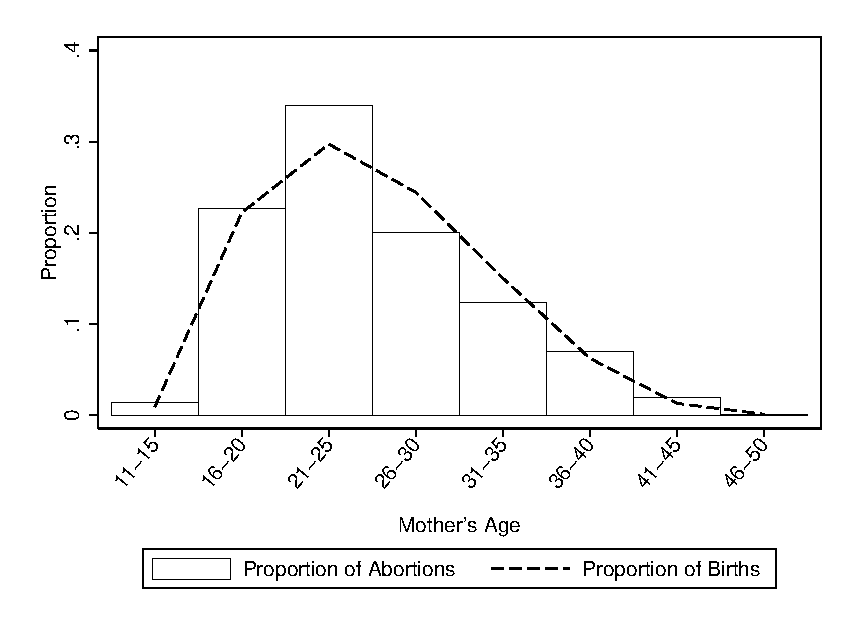
\includegraphics[scale=0.76]{figures/birthDescriptives.eps}
  \caption{Birth and Abortion Descriptives: Mexico}
  \label{MexBirthAbort}
  \vspace{2mm}
  \floatfoot{
    \textsc{Notes to figure}: Total births are plotted between 2001 and 2010.
    Abortions are plotted from the date of reform (April 26, 2007) until 2011.
    The total quantity of births is 22.20 million (all of Mexico), and total
    abortions are 69,861 (Mexico DF only).  Births are calculated from
    administrative data (INEGI) and abortions from administrative data (Secretary
    of Health, Mexico DF).}
\end{figure}


\restoregeometry
 
\begin{figure}[H]
\centering	\caption{Trends in Reform and non-Reform Areas}
\label{Trends}
\begin{subfigure}{.5\textwidth}
\centering	\caption{Trends in numbers of births}\label{birthTrends}
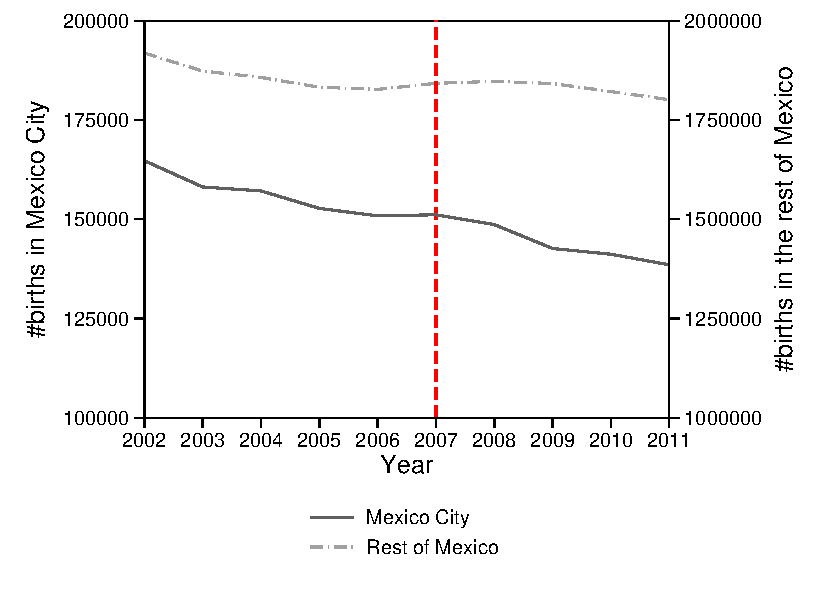
\includegraphics[scale=0.55]{figures/TrendBirth.pdf}
\end{subfigure}%
\begin{subfigure}{.5\textwidth}
\centering\caption{Trends in birth rates}\label{birthrateTrends}
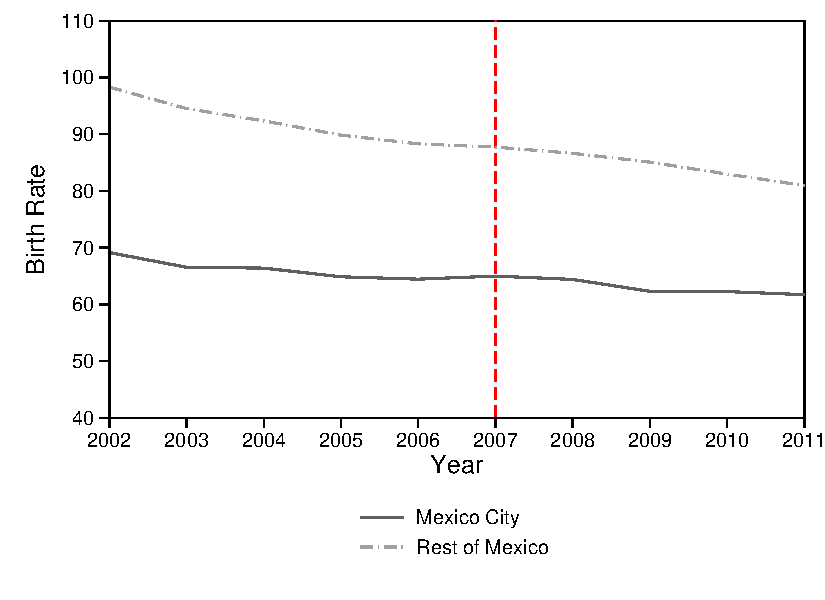
\includegraphics[scale=0.55]{figures/TrendBirthRates.pdf}
\end{subfigure}
\begin{subfigure}{.5\textwidth}
\centering	\caption{Trends in numbers of maternal deaths}	\label{deathsTrends}
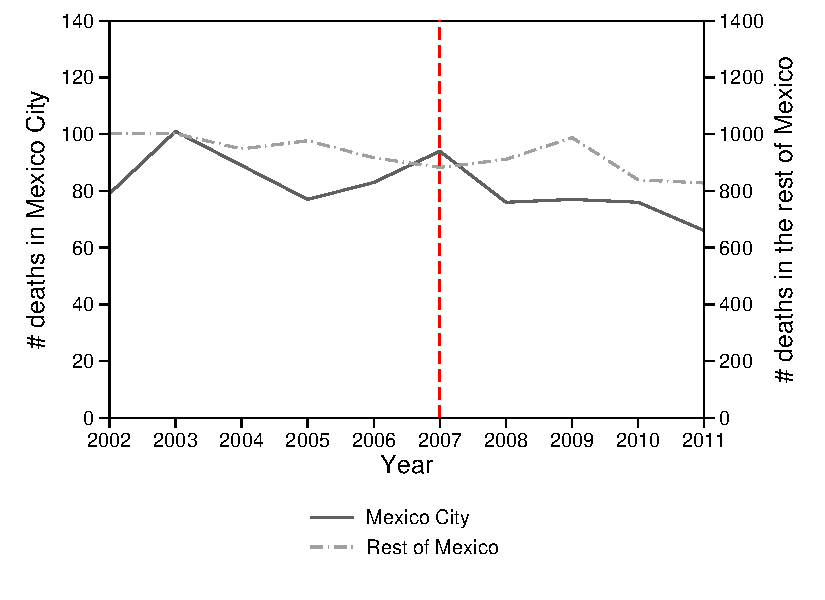
\includegraphics[scale=0.55]{figures/TrendMMR.pdf}
\end{subfigure}%
\begin{subfigure}{.5\textwidth}
\centering \caption{Trends in maternal mortality ratio}	\label{mmrTrends}
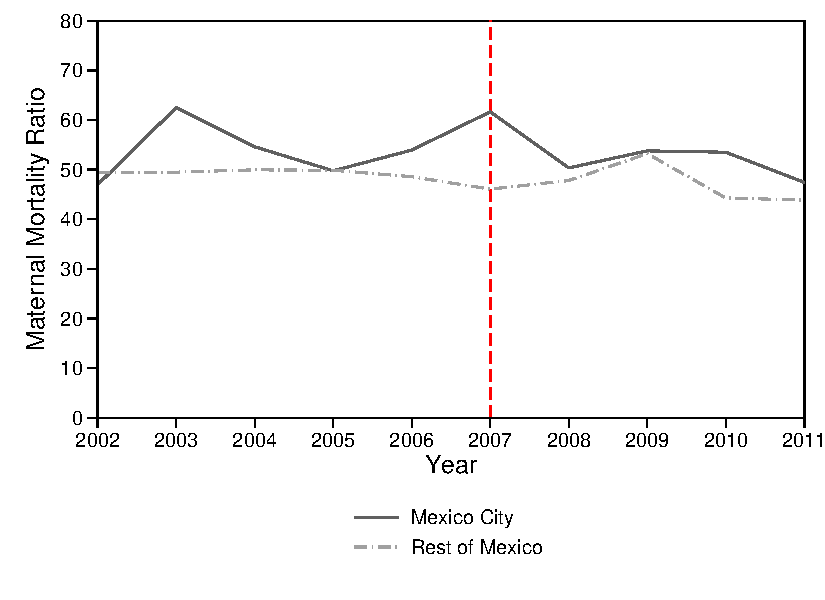
\includegraphics[scale=0.55]{figures/TrendMMratio.pdf}
\end{subfigure} 
\floatfoot{Note to Figure~\ref{Trends}: Each figure is constructed from administrative data made available by INEGI. Trends are constructed based on population weighted means for fertile aged women 15-44. The vertical dashed line represents the year of the reform. The State of Mexico is excluded due to potential spillover effects. In Figure a) trends in the number of births are displayed. In Figure b) trends in birth rates (the annual number of births per 1,000 women) are presented. In Figure c) the number of maternal deaths are presented followed by the trends in maternal mortality ratio (the annual number of deaths per 100,000 deaths) presented in Figure d). In Figure a) and c) the y-axis to the left shows the levels in Mexico City and y-axis to the right shows the levels in the rest of Mexico.}
 \end{figure}

 
\begin{figure}[H]
\centering	\caption{Placebo tests}
\label{placebo}
\begin{subfigure}{0.5\textwidth}
\centering	\caption{Event study, Fertility}	\label{placebo_birth}
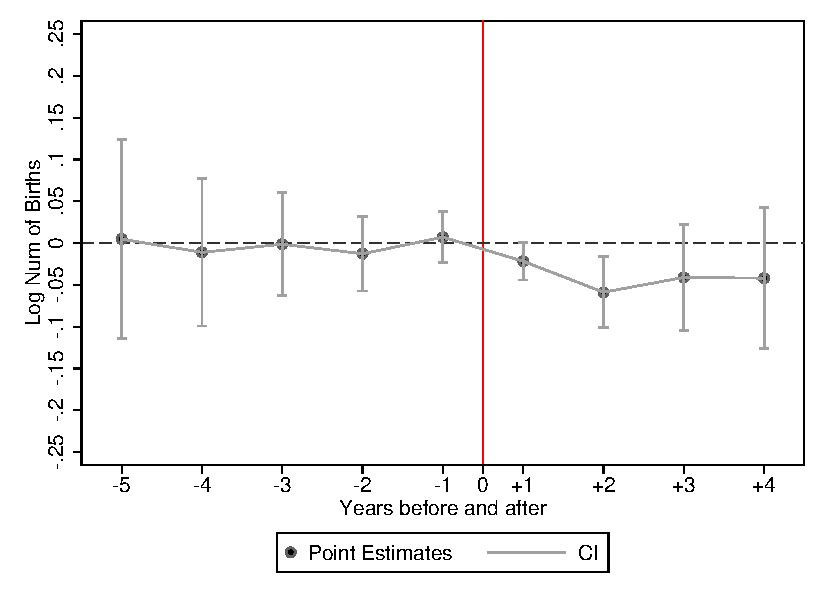
\includegraphics[scale=0.55]{figures/Placeboln_birth.pdf}
\end{subfigure}%
\begin{subfigure}{0.5 \textwidth}
\centering	\caption{Event study, Maternal mortality}	\label{placebo_mmr}
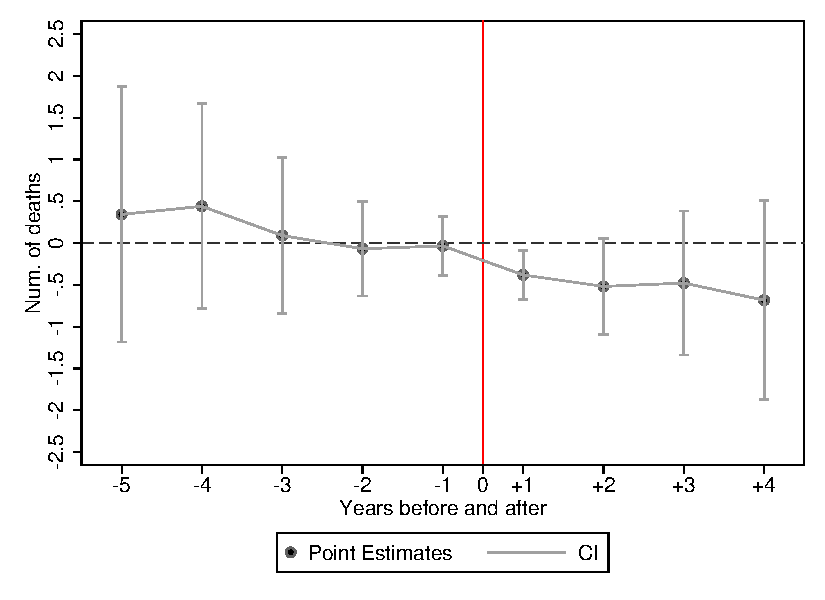
\includegraphics[scale=0.55]{figures/Placebommr.pdf}  	
\end{subfigure}
\floatfoot{Note to figure ~\ref{placebo}: The coefficient plot shows point estimates and confidence intervals estimated according to Equation~\eqref{eq2} using OLS regressions (Figure~\ref*{placebo_birth}) and Poisson regressions (Figure~\ref*{placebo_mmr}). The sample consists of all births and maternal deaths among women aged 15-44 for the period 2002-2011. Leads and lags (5 years before and 4 years after the reform) defined by interaction terms for each year and the treatment area (Mexico City) are included in order to examine anticipatory effects as well as post treatment effects for fertility (a) and maternal mortality (b) respectively. The year of the reform, 2007, is used as the baseline category. The State of Mexico is excluded due to potential spillover effects. A full set of fixed effects, time varying controls and state-specific linear time trends are included in each regression (see note to Table~\ref{heteroReg}). }
\end{figure} 

\begin{figure}[H]
\centering	\caption{Spillover Effects}	\label{SpilloverFigure}
\begin{subfigure}{0.5\textwidth}
\centering	\caption{Fertility}\label{spillover_birth}
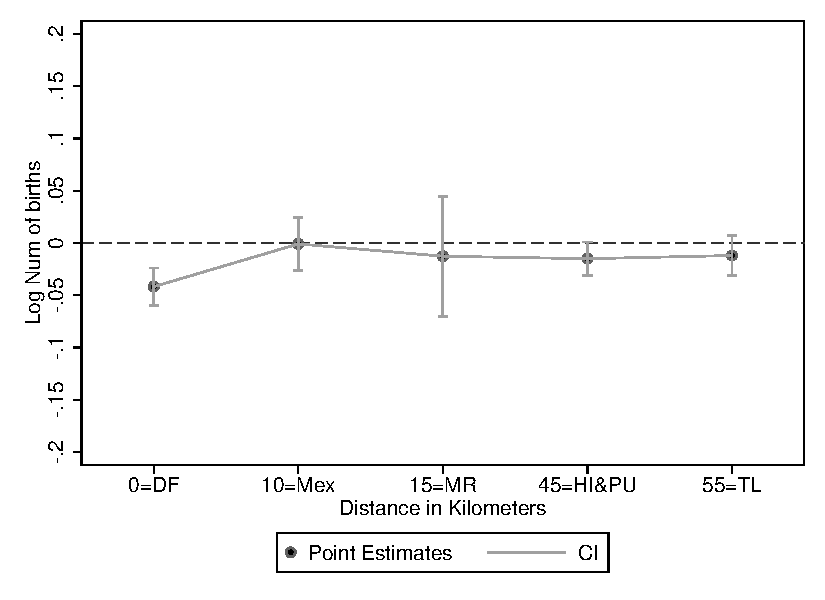
\includegraphics[scale=0.55]{figures/SpillOverBirth.pdf}
\end{subfigure}%
\begin{subfigure}{0.5 \textwidth}
\centering	\caption{Maternal mortality}\label{spillover_MMR}
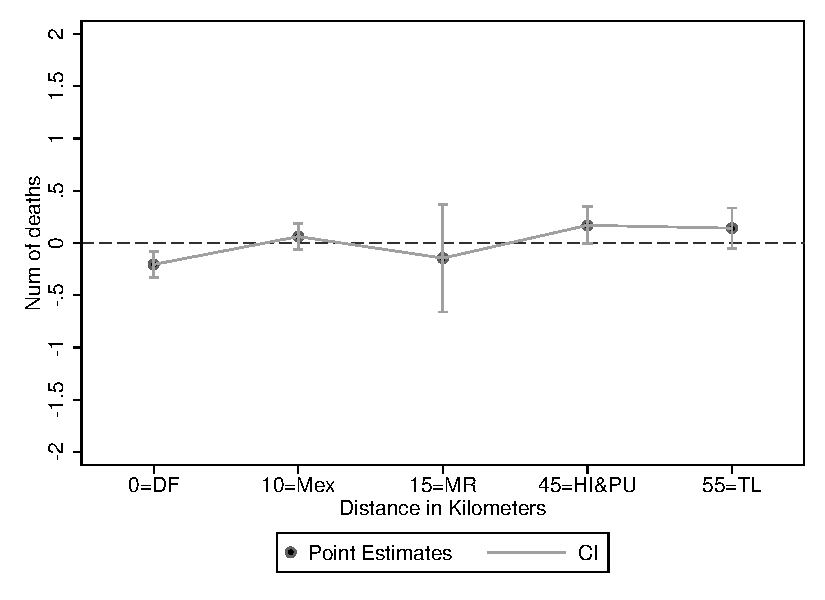
\includegraphics[scale=0.55]{figures/SpillOverMMR.pdf}
\end{subfigure}
\floatfoot{Note to figure ~\ref{SpilloverFigure}: The coefficient plot shows point estimates and confidence intervals estimated according to Equation~\eqref{eq3} using OLS regressions (Figure~\ref*{placebo_birth}) and Poisson regressions (Figure~\ref*{placebo_mmr}). The sample consists of all births and maternal deaths among women aged 15-44 for the period 2002-2011. The results are presented in Figure~\ref{spillover_birth} and~\ref{spillover_MMR}. We include multiple treatment variables equal to unity (9 months) after the law was passed for states with the minimum distance intervals 0-5, 6-10, 11-15 up to 51-55 to Mexico City, in order to examine spillover effects. A full set of fixed effects, time varying controls and state-specific linear time trends are included in each regression (see note to Table~\ref{heteroReg}).}
\end{figure} 
 



 
\end{spacing}
\end{document}
